\chapter{Algoritmos de visualización de SDFs}\label{cap:2}
Una vez estudiadas las técnicas a través de las cuales podemos crear y manipular primitivas, podemos usar estas para formar la escena que queremos representar. Podemos optar por dos enfoques. El primero de ellos es hacer \textit{spheretracing} una vez por cada primitiva que conforme la escena, lo cual permitiría tener un control más preciso sobre las propiedades de cada objeto de la escena de forma individual, como por ejemplo su apariencia (material) o distancia de dibujado. El otro enfoque consiste en combinar todas las primitivas de la escena en una sola mediante el operador booleano de unión. La principal ventaja en este caso sería el tener toda la escena definida a partir de una única SDF, de forma que tenemos la información más condensada y el renderizado es más sencillo al no tener que combinar el resultado de varias ejecuciones del algoritmo de \textit{spheretracing}. El precio a pagar por esta simplicidad es que perdemos el control más granular que sí teníamos antes. No obstante, optaremos por este último enfoque, tanto por simplicidad como porque nuestro objetivo final es crear nuevas superficies, y lo que más sentido tiene es que usemos una única SDF para representarlas.\newline

Ahora que tenemos definida la escena a partir de una función distancia con signo, necesitamos una forma de visualizarla. En IG se utilizan diferentes técnicas y algoritmos que transforman datos geométricos en otros que nuestras pantallas puedan representar. Dos de los métodos más utilizados son la rasterización y el trazado de rayos o \textit{raytracing}. En general, la rasterización es el método más usado para aplicaciones interactivas, ya que las GPUs fueron originalmente diseñadas para realizar rasterización de forma eficiente. Por otro lado, el \textit{raytracing} ofrece resultados más realistas, sobretodo en los aspectos relacionados con la iluminación, a precio de ser más lento. En los últimos años son cada vez más comunes las GPUs con soporte hardware para \textit{raytracing}, haciendo que se extienda su uso a aplicaciones interactivas, como los videojuegos.\newline

A la hora de trabajar con estos algoritmos es importante la forma en la que se representa la información de la geometría. La más común en rasterización y \textit{raytracing} es a través de mallas de polígonos, un conjunto de puntos de un espacio afín que forman caras planas. En ambos algoritmos necesitamos hacer uso del concepto de primitiva como los elementos más pequeños que pueden ser visualizados, y típicamente se trata de triángulos cuando se trabaja con mallas de polígonos. En nuestro caso no usamos mallas de polígonos, y tenemos una representación no discreta de la geometría de la superficie. Si bien la rasterización se puede adaptar para trabajar con objetos diferentes a mallas de polígonos, esto no es lo común, y el \textit{raytracing} es mucho más adaptable en estos casos, pues permite trabajar con cualquier tipo de objeto con el que se pueda calcular la intersección con un rayo, como ocurre con las SDFs.\newline

La \textbf{rasterización} recorre cada primitiva $P$ del modelo, comprobando para cada una qué conjunto $S$ de pixels de la pantalla la cubren. Una vez obtenidos los pixels, se ejecutará un programa escrito por el programador (\textit{fragment shader}) para cada uno de ellos, que calculará el color final del píxel. El funcionamiento del \textbf{\textit{raytracing}} es similar al de la rasterización, pero intercambiando los dos bucles. El procedimiento consiste por tanto en recorrer los pixels de la pantalla y comprobar qué primitivas del modelo cubren cada uno. Para ello se traza un rayo por el centro de cada píxel y se calcula la intersección con el objeto, razón del nombre \qq{trazado de rayos}. En la \autoref{fig:algVis} y la \autoref{fig:colorPixels} podemos apreciar las diferencias en el procedimiento de ambos algoritmos. Ambos métodos tienen complejidad algorítmica $\mathcal{O}(pn)$, siendo $n$ el número de primitivas y $p$ el de pixels, aunque en el caso del \textit{raytracing} esta se puede mejorar usando indexación espacial para la obtención del conjunto de primitivas que cubren cada píxel.\newline

\begin{figure}[ht!]
    \centering
    \begin{subfigure}[b]{0.47\textwidth}
        \begin{algorithm}[H]
            \caption{Rasterización}
            inicializar color de todos los pixels
            
            \For{cada primitiva $P$ en el modelo}{
                $S\gets $ pixels cubiertos por $P$

                \For{cada píxel $q$ en $S$}{
                    calcular color de $P$ en $q$

                    actualizar color de $q$
                }
            }
        \end{algorithm}
    \end{subfigure}%
    \hfill
    \begin{subfigure}[b]{0.47\textwidth}
        \begin{algorithm}[H]
            \caption{\textit{Raytracing}}
            inicializar color de todos los pixels
            
            \For{cada píxel $q$ de la pantalla}{
                $T\gets $ primitivas que cubren $q$

                \For{cada primitiva $P$ en $T$}{
                    calcular color de $P$ en $q$

                    actualizar color de $q$
                }
            }
        \end{algorithm}
    \end{subfigure}%
    \caption{Algoritmos de visualización}
    \label{fig:algVis}
\end{figure}

\begin{figure}[!ht]
     \begin{subfigure}[b]{0.98\linewidth}
        \centering
        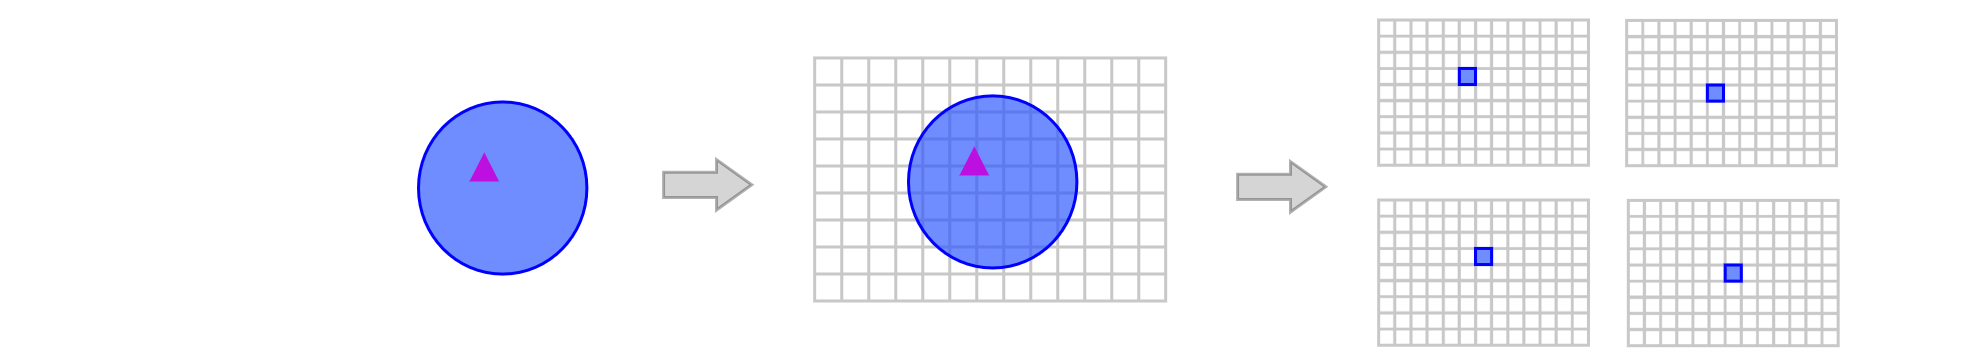
\includegraphics[width=0.9\textwidth]{Plantilla-TFG-master/img/rasterizacion.png}
        \caption{Rasterización}
     \end{subfigure}
     \begin{subfigure}[b]{0.98\linewidth}
        \centering
        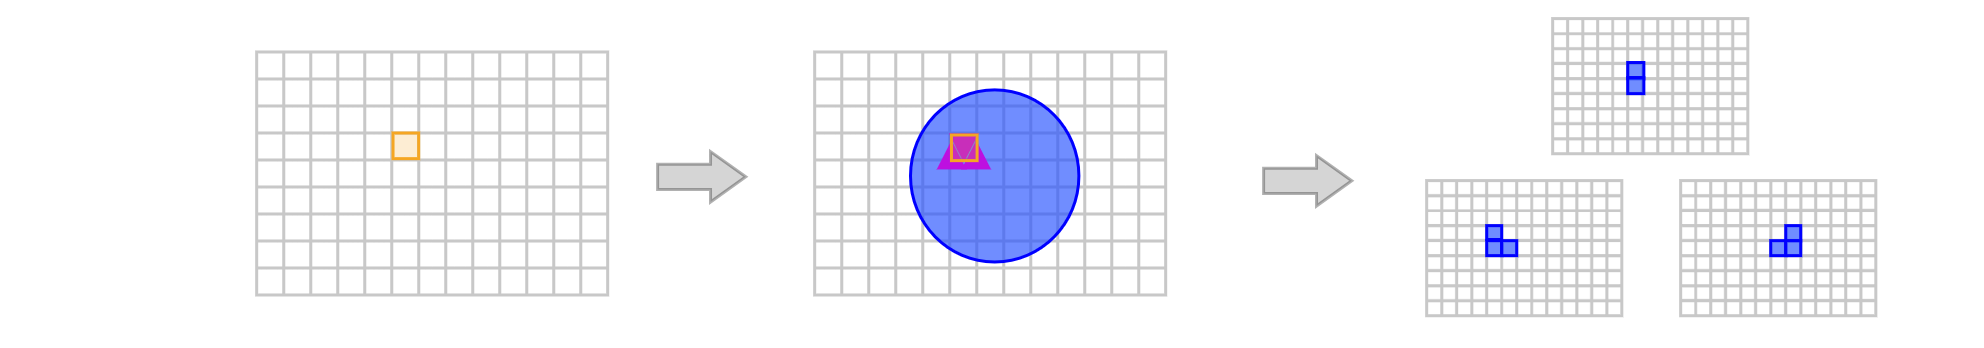
\includegraphics[width=0.9\textwidth]{Plantilla-TFG-master/img/raytracing.png}
        \caption{\textit{Raytracing}}
     \end{subfigure}
     \caption{Funcionamiento de los métodos de rasterización y \textit{raytracing}}
     \label{fig:colorPixels}
\end{figure}

Teniendo en cuenta las consideraciones anteriores, para representar superficies generadas por funciones distancia con signo  utilizaremos \textit{spheretracing}, un método basado en \textit{raytracing}. No obstante, para ello haremos uso de las APIs de rasterización en GPU, lo cual puede parecer contradictorio, pues como hemos visto ambos algoritmos tienen una estructura opuesta. El motivo fundamental de esta aparente contradicción es que las APIs de \textit{raytracing} solo están disponibles en GPUs modernas y avanzadas, y nosotros queremos poder realizar esta tarea en el mayor número de dispositivos posible. Podríamos conseguir esto realizando los cálculos en la CPU recorriendo secuencialmente los pixels, pero incluso paralelizándolos en varias hebras asignando a cada una un conjunto de pixels no podríamos conseguir el grado de interactividad que buscamos. La única solución es por tanto usar la GPU para realizar los cálculos de la intersección rayo-escena, pues son mucho más rápidas en este tipo de cálculos. Además, hoy en día prácticamente todos los dispositivos cuentan con GPUs, incluso los dispositivos móviles, y las APIs de rasterización son muy portables y conocidas. \newline

Para lograr nuestro objetivo de trazar rayos usando las APIs de rasterización usaremos que, como hemos visto, estas permiten ejecutar para cada píxel donde se proyecte una primitiva un código definido por el programador llamado \textit{fragment shader} y que produce el color del píxel. Así, en lugar de hacer \textit{raytracing} sobre una escena 3D, visualizaremos por rasterización un plano formado por dos triángulos cubriendo toda la imagen, lo que provocará la ejecución de una instancia del \textit{fragment shader} en cada píxel de la imagen, y será en él donde se implemente el algoritmo de intersección rayo-escena. A este plano lo llamaremos \textbf{lienzo} o \textit{canvas}, pues efectivamente estaremos pintando la escena encima suya píxel a píxel a través del \textit{fragment shader}.

\section{Renderizado por \textit{raytracing} en GPU usando un \textit{fragment shader}}\label{sec:render}
En esta sección estudiaremos en detalle el proceso de creación del lienzo usando una API cualquiera de rasterización y el desarrollo de los cálculos necesarios para ello , incluyendo la intersección del rayo con la escena, simulación avanzada de iluminación y técnicas de suavizado de la imagen.
\subsection{Creación del lienzo}\label{sec:lienzo} 
Cuando introdujimos el método de rasterización dijimos que este suele ser usado con mallas de polígonos, que a su vez estaban compuestas por puntos en un espacio afín que se unen formando caras. Lo cierto es que en IG se hace uso de múltiples espacios de coordenadas, los cuales es imprescindible conocer para entender el proceso de definición de geometría y pasamos a enumerar.
% Si bien se puede hacer \textit{raymarching} directamente sobre una escena 3D, nuestra escena constará únicamente de un plano formado por cuatro vértices y dos triángulos, que usaremos como lienzo  (o \textit{canvas}) para dibujar sobre él. Para ello, necesitaremos trabajar sobre diferentes espacios de coordenadas que pasamos a enumerar.
\begin{itemize}
    \item \textbf{Coordenadas locales o de objeto:} distancias relativas al origen del objeto.
    \item \textbf{Coordenadas globales o de mundo:} distancias relativas a un origen común para todos los objetos.
    \item \textbf{Coordenadas de cámara:} distancias relativas a un sistema de referencia posicionado y alineado con la cámara.
    \item \textbf{Coordenadas de recortado:} distancias normalizadas en el rango $[-1,1]^2$ relativas a un sistema asociado al rectángulo que forma la imagen en pantalla.
    \item \textbf{Coordenadas de dispositivo:} están centradas en la esquina inferior izquierda de la pantalla y toman valor en el rango $[0,r_x]\times [0,r_y]$, donde $r=(r_x,r_y)$ es la resolución de la pantalla.
\end{itemize}

% Si hacemos uso de \texttt{GL\_TRIANGLES} bastará con definir los vértices en sentido antihorario, pero hay que tener en cuenta que tendremos que repetir dos vértices, ya que se irán formando los triángulos en grupos de tres vértices. Una alternativa para no repetir vértices sería utilizar tablas de vértices e índices, pero en nuestro caso no merece la pena al tener únicamente seis vértices. Un ejemplo de definición de vértices formando un lienzo rectangular podría ser el que se muestra en la \autoref{fig:canvas}.\newline

% \begin{figure}[ht]
%     \centering
%     \begin{minipage}{0.50\textwidth}
%         \begin{lstlisting}
% glBegin(GL_TRIANGLES);
%     glColor3f(1.0f, 1.0f, 1.0f); 
    
%     // Triangulo inferior
%     glVertex3f(-2.0f, -1.0f, 0.0f);
%     glVertex3f(-2.0f, 1.0f, 0.0f);
%     glVertex3f(2.0f, 1.0f, 0.0f);
    
%     // Triangulo superior
%     glVertex3f(-2.0f, -1.0f, 0.0f);
%     glVertex3f(2.0f, 1.0f, 0.0f);
%     glVertex3f(2.0f, -1.0f, 0.0f);
% glEnd();
% \end{lstlisting}
%     \end{minipage}%
%     \hfill
%     \begin{minipage}{0.40\textwidth}
%         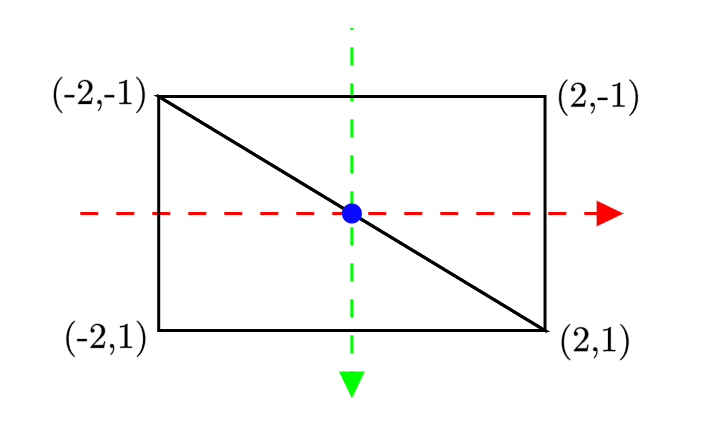
\includegraphics[width=\textwidth]{canvas.png}
%     \end{minipage}
    
    
%     \caption{Construcción del lienzo}
%     \label{fig:canvas}
% \end{figure}
Dado que para usar rasterización el lienzo deberá estar definido como una malla de polígonos, deberemos declarar los vértices que la conforman y cómo estos se unen formando primitivas, en este caso triángulos. Este lienzo, como toda geometría, tendrá asignado dos \textit{shaders} o procesadores, que son programas que se ejecutan en la GPU. Estos programas pueden recibir parámetros, pero son independientes entre sí, siendo la única forma en la que pueden comunicarse entre ellos mediante el paso de atributos de entrada y salida. Hay dos tipos de \textit{shaders}: de vértices (\textit{vertex shader}) y de fragmentos o pixels (\textit{fragment shader}), cada uno con atributos específicos de entrada y salida.\newline

En el \textit{vertex shader} utilizaremos los siguientes atributos.
\begin{itemize}
    \item $v_{loc}$: vector de cuatro flotantes que contiene las coordenadas
    homogéneas locales del vértice a procesar. La cuarta componente es la componente homogénea, que es necesaria para realizar el cambio a coordenadas recortadas. Se trata de un parámetro de entrada enviado por la aplicación al visualizar una secuencia de vértices.
    \item $v_{wc}$: vector de cuatro flotantes con la posición transformada del vértice actual. El objetivo del \textit{vertex shader} es el de calcular su valor, luego es un parámetro de salida. 
    % \item \textbf{\texttt{in vec4 gl\_Vertex}}: contiene las coordenadas locales del vértice actual y es pasado autómaticamente por la aplicación. 
    % \item \textbf{\texttt{out vec4 gl\_Position}}: posición transformada del vértice actual que deberemos calcular. La cuarta componente es la componente homogénea, que es necesaria para realizar el cambio a coordenadas recortadas.
\end{itemize}
Por otro lado, en el \textit{fragment shader} usaremos los que siguen.
\begin{itemize}
    \item $v_{frag}$: vector de cuatro flotantes con las coordenadas de dispositivo para el centro del píxel actual. Es un atributo de entrada, los cuales interpolan su valor automáticamente en cada vértice en los \textit{fragment shaders}. La cuarta componente es la inversa de la componente homogénea de $v_{rec}$, y se utiliza en el cálculo de la profundidad de los pixels y en las operaciones de corrección de perspectiva.
    \item $v_{col}$: terna RGBA de flotantes que contendrá el color del píxel actual. Es un parámetro de salida, y la función del \textit{fragment shader} es otorgarle un valor.
    % \item \textbf{\texttt{in vec4 gl\_FragCoord}}: coordenadas de dispositivo para el centro del píxel actual en el \textit{fragment shader}. Al ser un atributo de entrada del \textit{fragment shader}, está interpolada en cada vértice. La cuarta componente es la inversa de la componente homogénea de \texttt{gl\_Position}, y se utiliza en el cálculo de la profundidad de los pixels y en las operaciones de corrección de perspectiva.
    % \item \textbf{\texttt{out vec4 gl\_FragColor}}: terna RGBA que asignaremos como color del píxel actual en el \textit{fragment shader}.
\end{itemize}
% Adicionalmente, podremos pasar nuestros propios atributos desde otro programa si estos son de cierto tipo
% Por último, en caso de que queramos pasar nuestros propios atributos desde otro programa, deberemos hacerlo a través de un \texttt{uniform}.\newline

En primer lugar se ejecuta una instancia del \textbf{procesador de vértices o \textit{vertex shader}} para cada vértice de la geometría. Su finalidad es realizar transformaciones de coordenadas, y adicionalmente pasar atributos al \textit{fragment shader}. Dada la posición del vértice actual, que se nos proporciona a través del atributo $v_{loc}$, para cambiar de un sistema de coordenadas a otro se utilizan matrices de transformación \cite{article:matrices} \cite{article:matrices2}. Todas ellas son de flotantes con dimensión $4\times 4$, y haremos uso de las siguientes.
\begin{figure}[h]
    \centering
    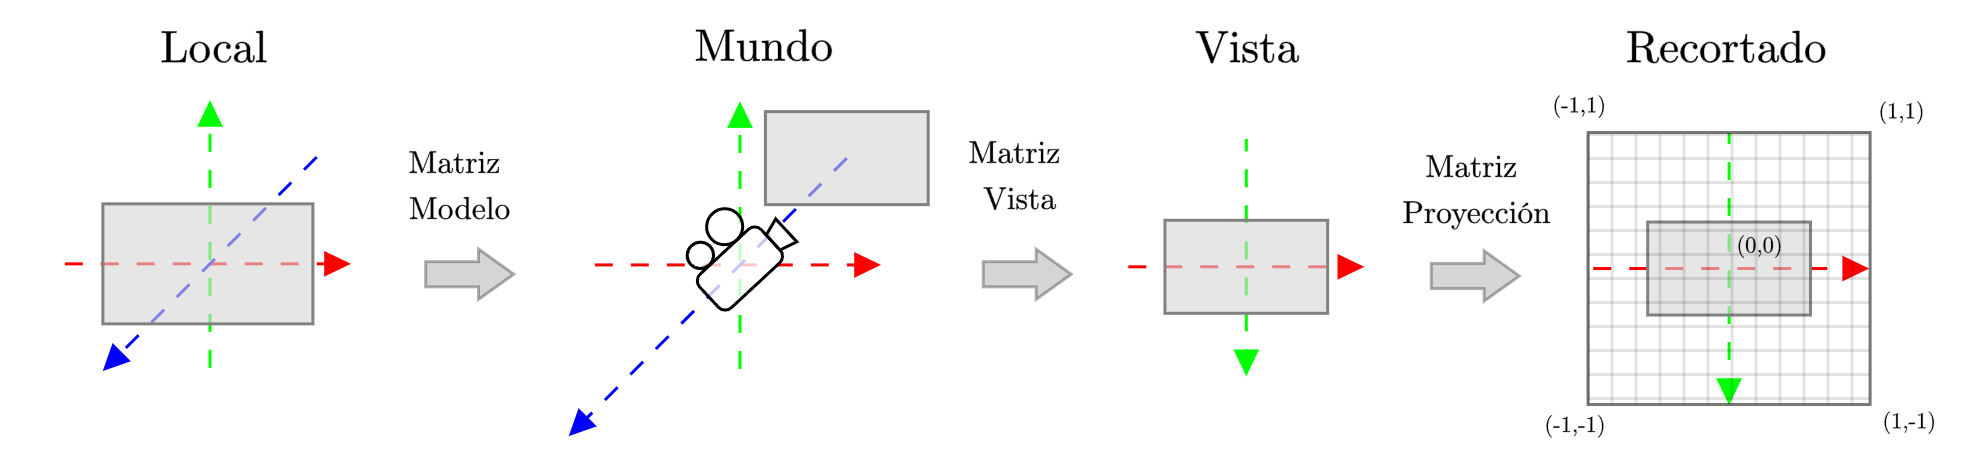
\includegraphics[width=\textwidth]{Plantilla-TFG-master/img/matrices2.png}
    \caption{Coordenadas locales a recortadas}
    \label{fig:matrices}
\end{figure}
\begin{itemize}
    \item \textbf{Matriz de modelo $\boldsymbol{M}$:} define la posición, orientación y escala del objeto en la escena. Se utiliza para pasar del coordenadas locales a coordenadas de mundo. En nuestro caso, si creamos el plano centrado en el origen, podemos simplemente tomar la matriz identidad de dimensión cuatro
    \begin{equation*}
        M = Id_{4\times 4}.
    \end{equation*}
    \item \textbf{Matriz de vista  $\boldsymbol{V}$:} define la posición y orientación de cada punto respecto a la cámara de la escena. Se utiliza para pasar de coordenadas de mundo a coordenadas de vista. Lo que ocurre en realidad es que la cámara está fija en el origen, y es el resto de la escena es la que se mueve respecto a ella. Por tanto, esta matriz contiene la posición y orientación inversa de la cámara. En nuestro caso, si queremos desplazar la cámara una unidad en el eje Z, la matriz de vista tendrá la forma
    \begin{equation*}
        V = \begin{pmatrix}
        1 & 0 & 0 & 0\\
        0 & 1 & 0 & 0\\
        0 & 0 & 1 & -1\\
        0 & 0 & 0 & 1
        \end{pmatrix}.
    \end{equation*}
    
    \item \textbf{Matriz de proyección:} define cómo la escena se proyecta en la pantalla, incluyendo el campo de visión, aspecto y planos cercano y lejano. Se utiliza para pasar de coordenadas de vista a coordenadas recortadas en función de las siguientes características del \textit{view-frustum}, la región del espacio de la escena que es visible por pantalla.
    \begin{itemize}
        \item Apertura vertical del campo de visión $\beta$ indicada como un ángulo entre $0$ y $180$ grados.
        \item Relación de aspecto $a$ entre el ancho $w$ y el alto $h$ del \textit{view-frustrum}.
        \item Límites cercano y lejano en el eje $Z$ cambiados de signo $n$ y $f$ del \textit{view-frustrum}.
    \end{itemize}
    La matriz se construye como
    \begin{equation*}
        M_P = \begin{pmatrix}
        \frac{c}{a} & 0 & 0 & 0\\
        0 & c & 0 & 0\\
        0 & 0 & \frac{n+f}{n-f} & \frac{2nf}{n-f}\\
        0 & 0 & -1 & 0
        \end{pmatrix}, \text{ donde } c = \coth\left({\frac{\beta}{2}}\right).
    \end{equation*}

    % \item \textbf{Matriz de ventana o \textit{viewport}:} se transforman las coordenadas de recortado a las coordenadas de dispositivo. Estas coordenadas están centradas en la esquina inferior izquierda de la pantalla y están en el rango $[0,r_x]\times [0,r_y]$, donde $r=(r_x,r_y)$ es la resolución de la pantalla.
\end{itemize}

\begin{figure}[ht!]
    \centering
    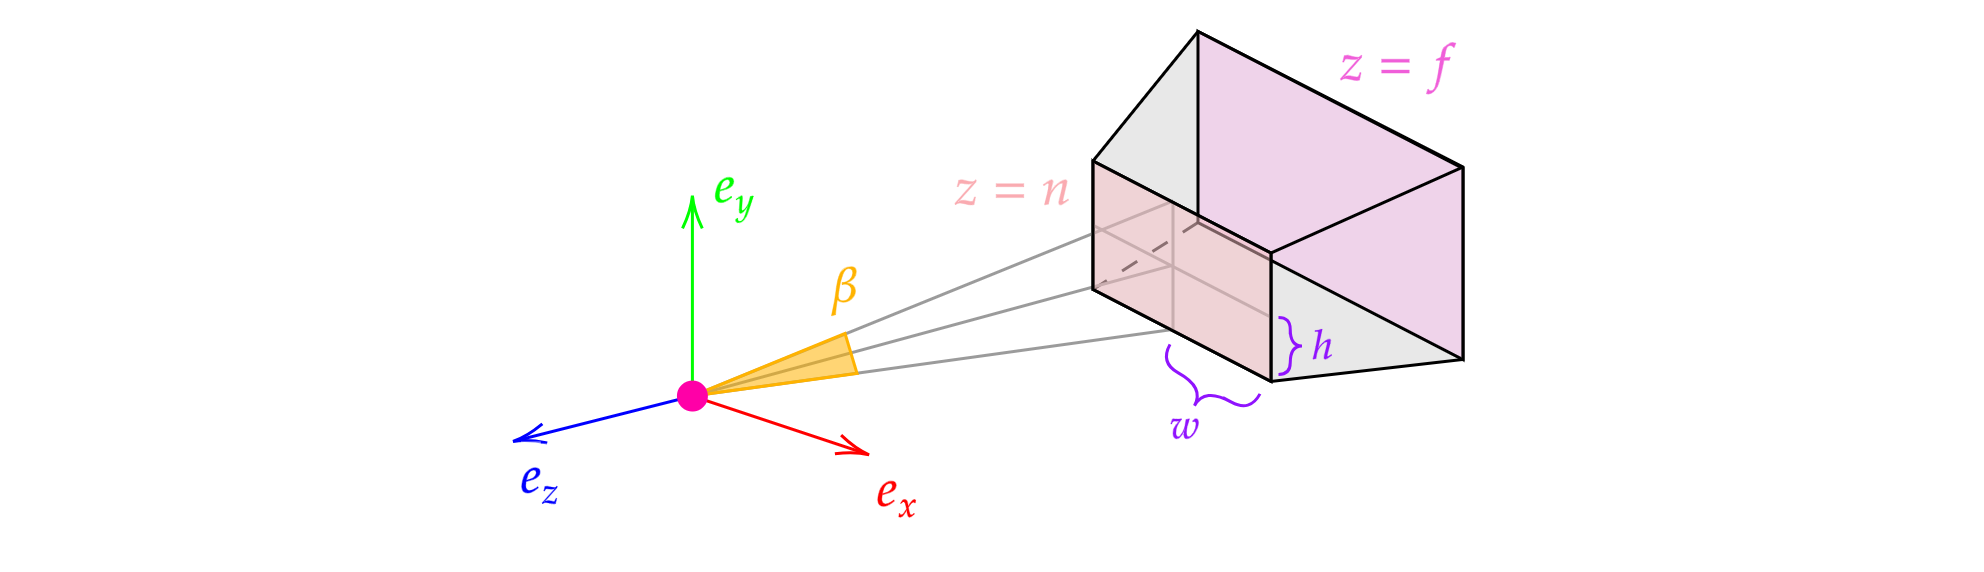
\includegraphics[width=\textwidth]{Plantilla-TFG-master/img/frustrum.png}
    \caption{Parámetros del \textit{view frustrum}}
\end{figure}

Con esta información ya podemos escribir nuestro \textit{vertex shader}, mostrado en la \autoref{fig:mainVS}.  
\begin{figure}[ht!]
    \centering
       \begin{algorithm}[H]
            \caption{Vertex Shader}
            \KwData{matriz de proyección $M_P$, matriz de vista $M_V$, matriz de modelo $M_M$, y coordenadas locales homogéneas del vértice $v_{loc}$}
            \KwResult{posición transformada del vértice actual en coordenadas homogéneas de mundo $v_{wc}$}
                $v_{wc} \gets M_P \cdot M_V \cdot M_M \cdot v_{loc}$
        \end{algorithm}
    \caption{Cuerpo del método \texttt{main} del \textit{vertex shader}}
    \label{fig:mainVS}
\end{figure}

Tras la ejecución del \textit{vertex shader} las coordenadas de recortado se transforman a coordenadas de dispositivo, que el \textbf{procesador de fragmentos o \textit{fragment shader}} recibirá como entrada. De él se ejecutará una instancia para cada píxel de la pantalla, y su objetivo es asignar a la variable $v_{loc}$ el color que el píxel tendrá como una terna RGBA, y será aquí donde hagamos todos los cálculos necesarios pare renderizar la superficie con \textit{spheretracing}. El primer paso para esto será definir un sistema de coordenadas dentro del propio lienzo con el que sea más cómodo trabajar que con el que ya disponemos a través de $v_{frag}$.\newline

Para obtener estas coordenadas, primero desplazamos el origen que nos proporciona $v_{frag}$ al centro de la pantalla usando el número de columnas y filas de pixels en la imagen, que deberemos pasar como parámetro al \textit{shader} y llamaremos \texttt{u\_resolution}, para posteriormente normalizar respecto a alguno de los ejes. Hacemos esto porque si intentamos normalizar sobre ambos ejes obtendremos coordenadas en el rango $[-0.5,0.5]^2$, y al no ser (en general) el lienzo cuadrado, la imagen se verá estirada en la dirección del eje más largo. Nosotros normalizaremos respecto al eje vertical, ya que en nuestro caso será siempre el menor. Esto nos dará como resultado unas coordenadas con valores en $\left[ -0.5\cdot aspect, 0.5\cdot aspect \right] \times [-0.5, 0.5]$, donde $aspect$ es el ratio de aspecto del lienzo, el resultado de dividir el ancho de la imagen por el alto, ambos medidos en pixels. Finalmente, para que la coordenada Y tome siempre valores en $[-1,1]$ multiplicamos por dos. Con esto conseguimos las coordenadas del centro del pixel en coordenadas normalizadas de dispositivo, similares a las de recortado pero divididas por la componente homogénea.
\begin{equation*}
    uv = \frac{2\cdot(v_{frag} - 0.5\cdot u\_resolution)}{u\_resolution_y}.
\end{equation*}

Hemos denotado a las coordenadas obtenidas como $uv$, haciendo referencia a la similitud que tienen con el uso que se le da a las coordenadas de textura habituales, ya que las vamos a usar para pintar sobre el lienzo como si de aplicar una textura se tratase. Cuando se trabaja con \textit{fragment shaders} la forma de debugear es dando colores a los pixels. En nuestro caso, podemos ver la diferencia entre ambos sistemas de coordenadas si usamos $uv$ como los canales rojo y verde del parámetro de salida $v_{col}$, superponiendo una rejilla construida usando la función módulo para apreciar si existe deformación, tal y como se muestra en la \autoref{fig:uv}. En ella podemos observar que si normalizamos sobre el eje horizontal, los verdes y amarillos no llegan a ser del todo intensos, ya que la componente del verde (la vertical) no llega a su valor máximo. Normalizando ambos ejes obtenemos el rango de colores completo, pero existe deformación en la rejilla debido a que el lienzo no es cuadrado. Finalmente, normalizando sobre el eje vertical obtenemos también el rango completo de colores, ya que los valores del eje horizontal que se salen del rango $[-1,1]$ son visualizados como si hubieran sido acotados en dicho intervalo, pero la rejilla se dibuja correctamente. En las siguientes secciones veremos cómo usar estas coordenadas para dibujar nuestra superficie sobre el lienzo.
\newline

\begin{figure}[htbp]
    \centering
    \begin{minipage}[b]{0.45\textwidth}
        \centering
        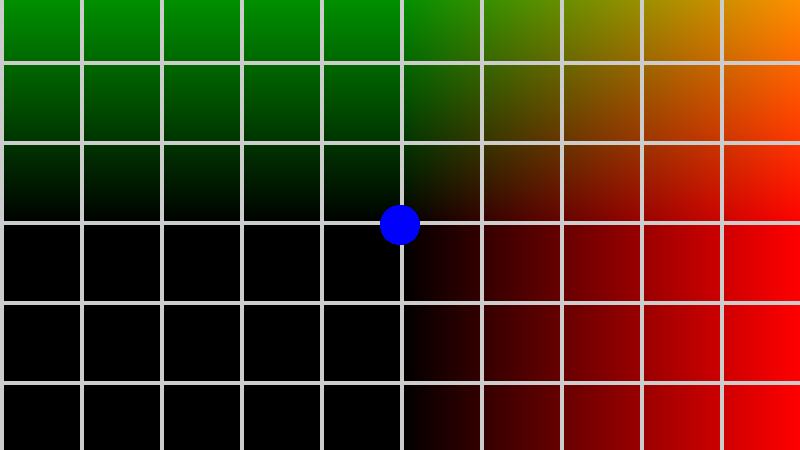
\includegraphics[width=\textwidth]{Plantilla-TFG-master/img/normX.png}
        \caption{Eje X}
    \end{minipage}
    \hfill
    \begin{minipage}[b]{0.45\textwidth}
        \centering
        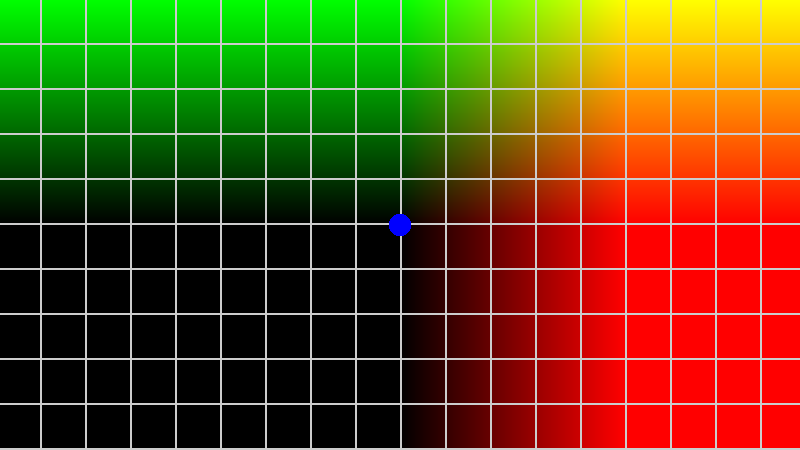
\includegraphics[width=\textwidth]{Plantilla-TFG-master/img/normY.png}
        \caption{Eje Y}
    \end{minipage}
    
    \medskip
    
    \begin{minipage}[b]{0.45\textwidth}
        \centering
        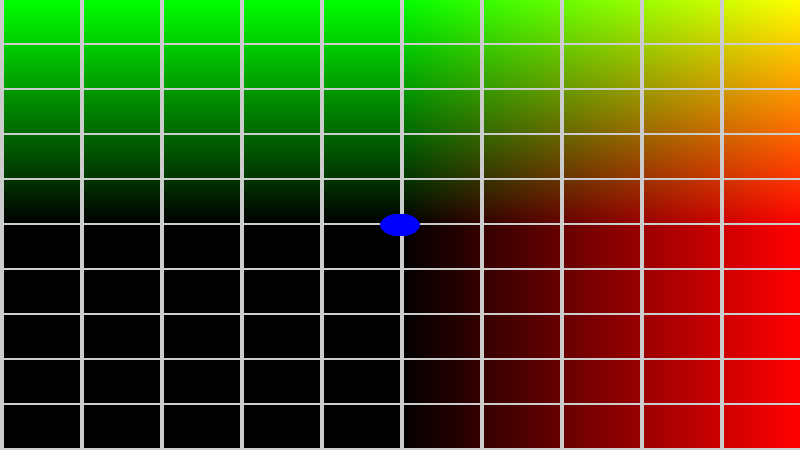
\includegraphics[width=\textwidth]{Plantilla-TFG-master/img/normXY.png}
        \caption{Ejes X e Y}
    \end{minipage}
    
    \caption{Normalización de coordenadas sobre distintos ejes}
    \label{fig:uv}
\end{figure}


\subsection{Generación de rayos primarios}
A partir de ahora, pensamos en nuestra escena no como en la que hemos definido el lienzo, sino aquella que queremos dibujar usando \textit{spheretracing} dada una función distancia con signo $\phi$. Esta escena estará definida en el espacio de coordenadas de mundo, el cual tiene un marco de referencia formado por tres vectores unitarios $B=\{e_x,e_y,e_z\}$ y un origen $o$, y colocaremos en ella los siguientes elementos (a partir de ahora supondremos que todas las tuplas de coordenadas son en coordenadas de mundo):
\begin{itemize}
    \item La \textbf{isosuperficie} $S_{\phi}$.
    \item \textbf{Plano de visión:} rejilla perpendicular al eje óptico de la cámara, donde cada uno de sus cuadrados corresponde a un píxel del lienzo.
    \item \textbf{Punto de la cámara $\boldsymbol{c_o}$:} punto del espacio desde donde se observa la escena.
    \item \textbf{Punto de atención o \textit{lookat point} $\boldsymbol{l}$:} hacia que punto del espacio debe mirar la cámara. En general tomaremos $l=o=(0,0,0)$.
\end{itemize}
La idea para conseguir representar la superficie consiste en trazar rayos a partir de $c_o$ hacia el centro de cada uno de los cuadrados del plano de visión, cada uno representando un píxel de la pantalla, de forma que si el rayo interseca con $S_\phi$ significa que ese píxel corresponde a un punto de la superficie, y será coloreado como tal.
\begin{figure}[h]
    \centering
    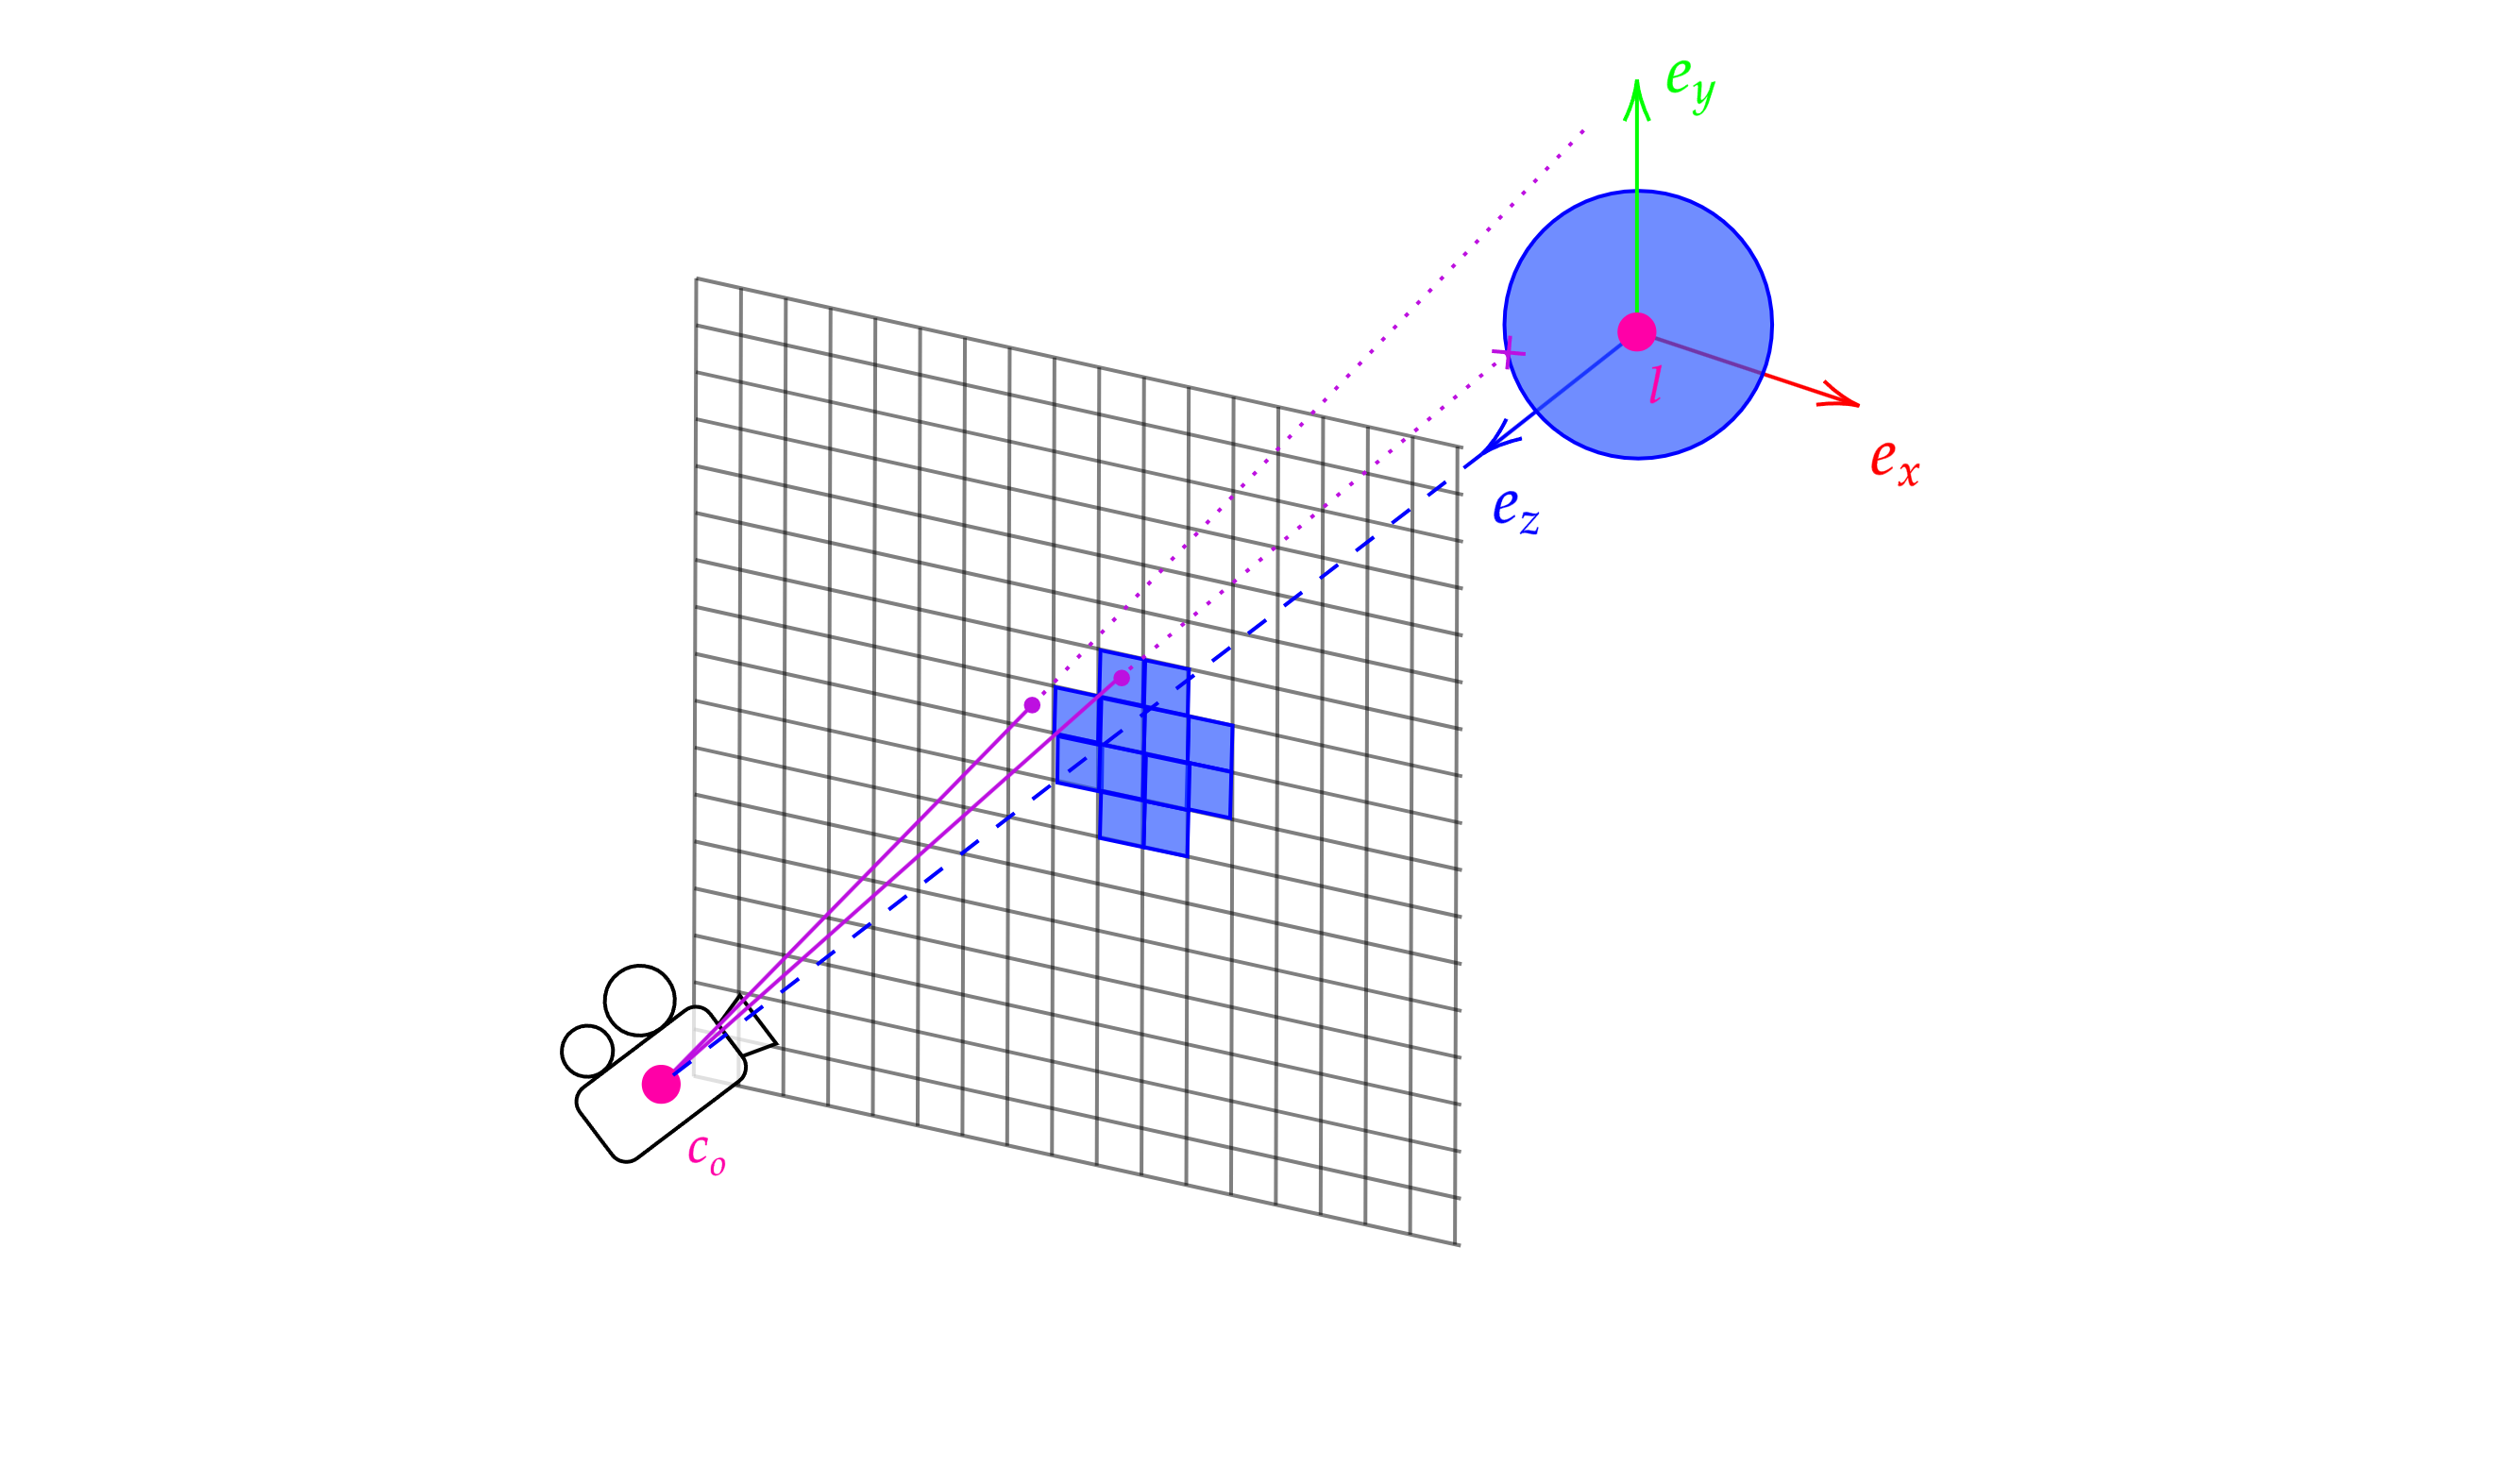
\includegraphics[width=\textwidth]{Plantilla-TFG-master/img/raymarch_fix.png}
    \caption{Trazado de rayos a través del plano de visión}
    \label{fig:raymarch1}
\end{figure}
\newline

Cada uno de estos rayos estará definido por un origen $r_o$ y una dirección $r_d$. El origen será siempre la posición de la cámara $c_o$, pero obtener la dirección requiere más trabajo. En el escenario descrito en la \autoref{fig:raymarch1}, donde $S_{\phi}$ es una esfera centrada en el origen y el observador se encuentra sobre el eje Z, dado que en todo momento conocemos las coordenadas de cada punto de la rejilla a través de $uv = (u,v)$, es claro que podemos tomar
$$r_d = (u,v,0) - c_0.$$ 
Una opción sería tomar $c_0 = (0,0,d)$, donde el valor $d$ es la distancia desde el punto del observador (foco de la proyección) al plano de visión. Modificar el valor de $d$ cambiaría los ángulos de apertura de visión horizontal y vertical, cambiando el tamaño aparente de los objetos proyectados. Es decir, $d$ actuaría como un control del campo de visión, de forma que cuanto mayor sea su valor mayores serán los ángulos de visión, y por tanto los objetos se verán más pequeños. Lo fijaremos a un valor de $1$. Sin embargo este escenario es el más sencillo posible, y si queremos poder mover la cámara manteniendo el punto de atención $l$ en el centro de la pantalla tendremos que poder trabajar con una orientación arbitraria suya. Para ello deberemos construir un marco de coordenadas de vista relativo a la cámara, que definiremos por una base ortonormal $\{f_1,f_2,f_3\}$ y el origen $c_0$.\newline

Para obtener el valor de los elementos de $f_1,f_2$ y $f_3$ empezamos obteniendo los siguientes vectores ortonormales.
\begin{itemize}
    \item \textbf{Vector director $\boldsymbol{c_d}$:} indica la dirección hacia la que mirará la cámara, que será paralela al eje $Z$ del marco de coordenadas de vista. Su valor vendrá dado por $c_d = l-c_o$.
    \item \textbf{\textit{Right vector} $\boldsymbol{c_r}$ }: paralelo al eje $X$ del marco de coordenadas de vista. Debe ser perpendicular tanto a $c_d$ como al vector \textit{view-up}. Este último, que denotaremos como $u$, es un vector libre que indica la dirección que el observador verá proyectada en vertical y apuntando hacia arriba en la imagen, y normalmente se toma el valor $u=(0,1,0)$ para que coincida con el eje $Y$. Al ser $c_r$ perpendicular al vector director y a \textit{view-up}, podemos obtenerlo como el producto vectorial de ambos: $c_r = u \times c_d$.
    \item \textbf{\textit{Up vector} $\boldsymbol{c_u}$}: paralelo al eje $Y$ del marco de coordenadas de vista. Como debe ser ortogonal a los otros dos, lo calculamos como $c_u = c_d\times c_r$.
\end{itemize}
A partir de estos vectores podemos obtener $\{f_1,f_2,f_3\}$ normalizándolos y teniendo en cuenta que el plano de visión y la cámara estarán orientados de forma opuesta:
\begin{equation*}
    f_1 = -\frac{c_r}{\Vert c_r\Vert} = -\frac{(0,1,0)\times c_d}{\Vert l-c_o\Vert},\quad 
    f_2 = \frac{c_u}{\Vert c_u\Vert } = f_3\times f_1, \quad
    f_3 = -\frac{c_d}{\Vert c_d\Vert} = -\frac{l-c_o}{\Vert l-c_o\Vert}. 
\end{equation*}
Ahora que tenemos el nuevo marco cartesiano, queda transformar el vector director original $r_d = (u,v,-1)$ a la base que acabamos de obtener. La matriz de cambio de base serán las coordenadas por columnas de $\{f_1,f_2,f_3\}$ escritas en función de $\{e_x,e_y,e_z\}$, que al ser la base del marco de coordenadas de mundo y al tratarse de una matriz de cambio de base entre dos marcos cartesianos, coincidirá con escribir por columnas $\{f_1,f_2,f_3\}$, de forma que
\begin{equation*}\label{eq:rayo}
    rayo = (u,v,-1)_{B}^t = \big(f_1\ \vert\  f_2\  \vert\  f_3\big) \cdot \begin{pmatrix}
        u\\
        v\\
        -1
    \end{pmatrix}.
\end{equation*}

\begin{figure}[ht!]
    \centering
    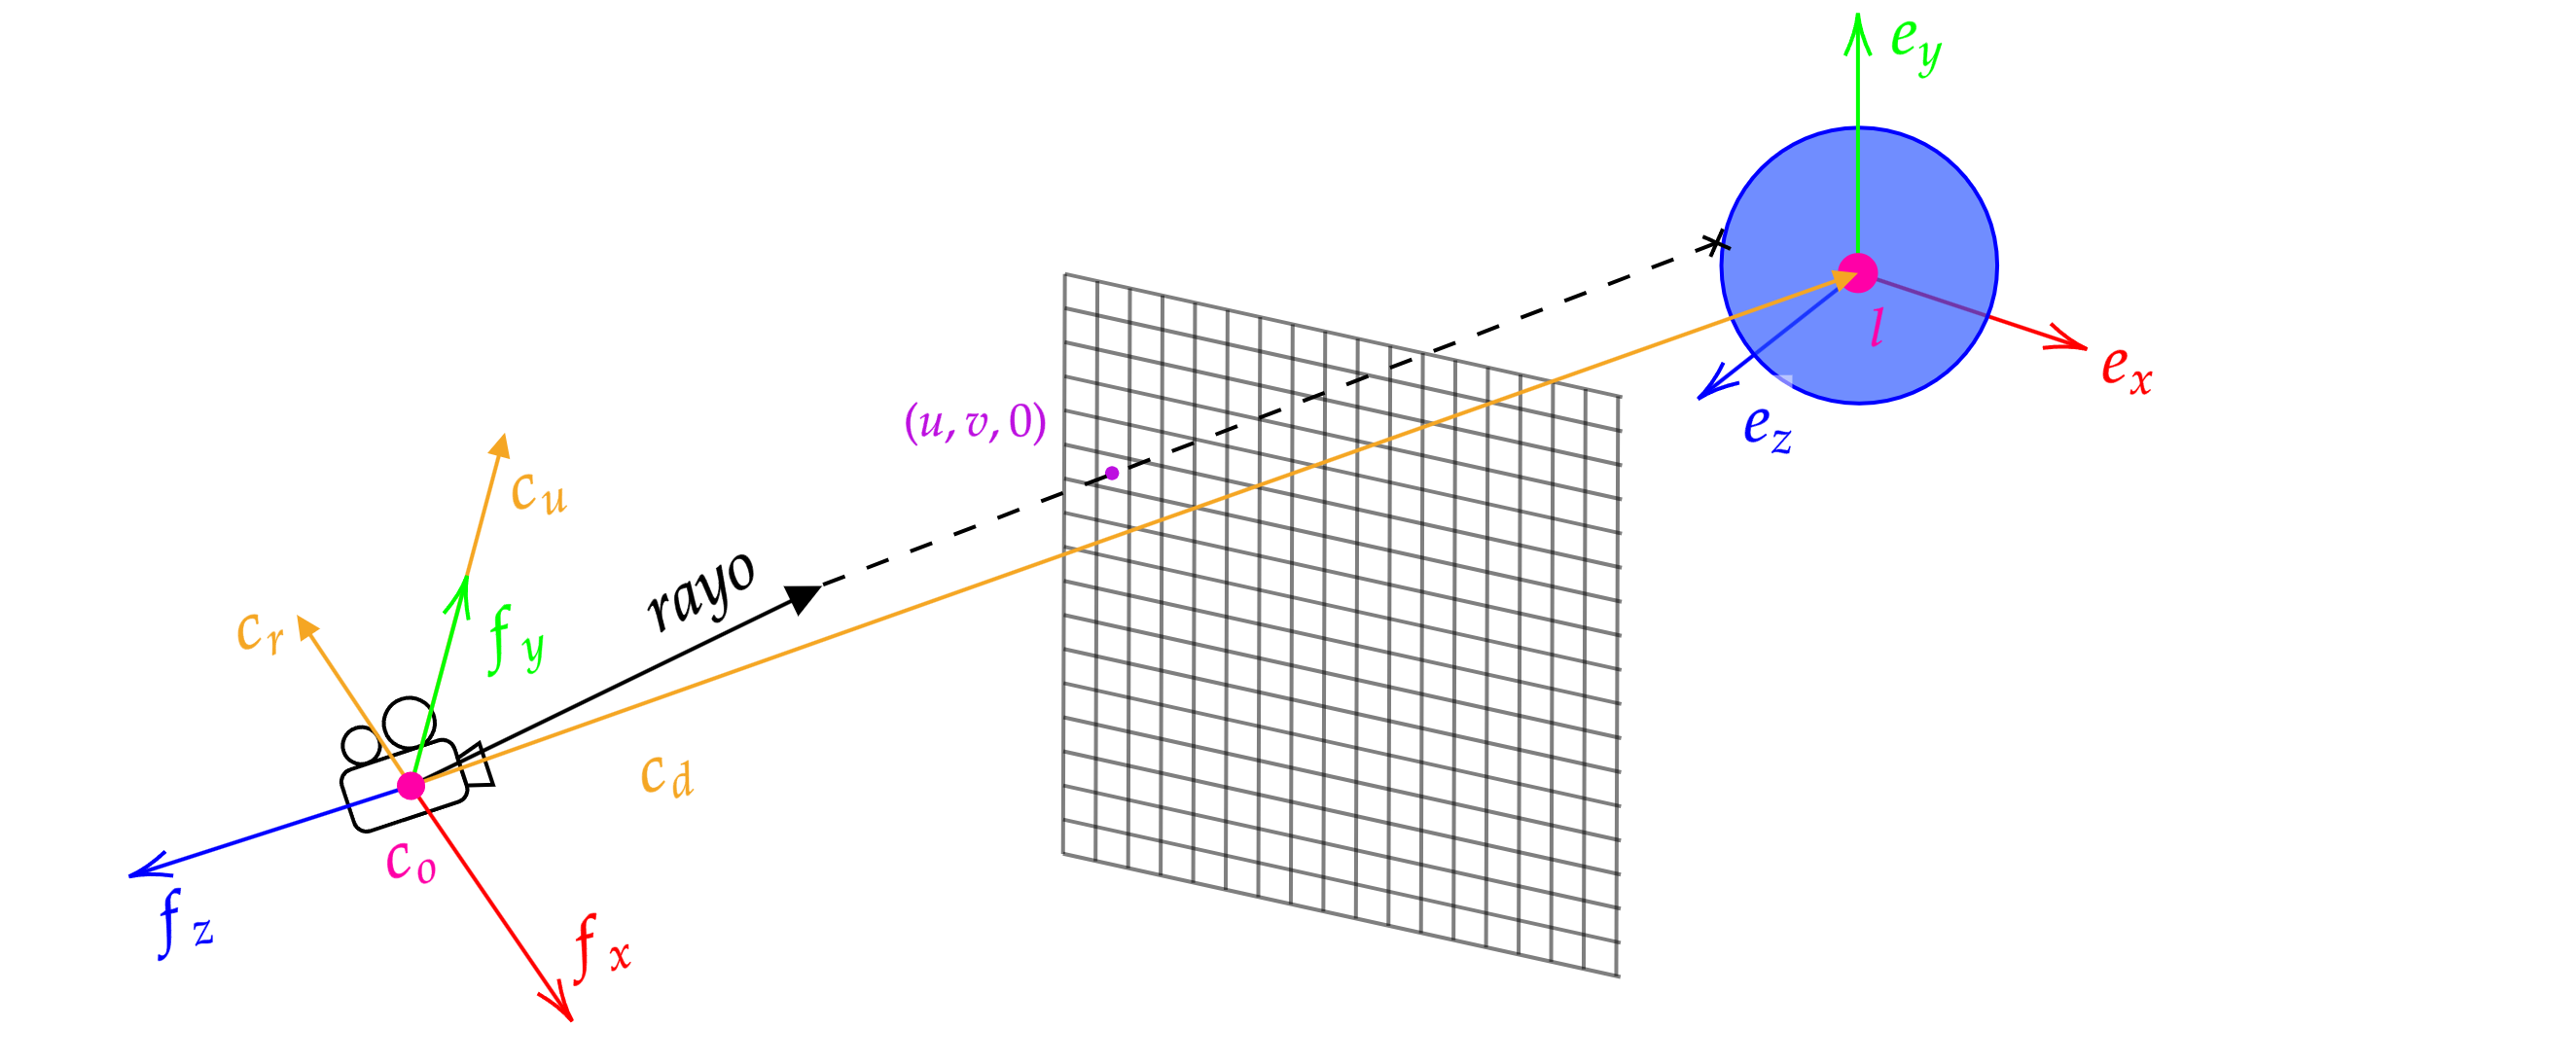
\includegraphics[width=\textwidth]{Plantilla-TFG-master/img/raydir_fix.png}
    \caption{Obtención de la dirección del rayo}
    \label{fig:raydir}
\end{figure}

\subsection{Algoritmos de intersección rayo-escena: \textit{raymarching} y \textit{spheretracing}}\label{sec:tracing}
Una vez que conocemos toda la información del rayo ya estamos en disposición de comprobar si este interseca con $S_{\phi}$. Para esto se pueden utilizar varios algoritmos, de entre los que estudiaremos el \textit{raymarching} y el \textit{spheretracing}. El método del \textit{spheretracing} es una variante del \textit{raymarching}, así que estudiaremos este primero.\newline

El \textbf{\textit{raymarching}} es un método iterativo: a partir de $c_o$, en cada iteración avanzamos en la dirección del rayo una distancia fija $\delta$. Evaluamos entonces nuestra SDF en la posición actual, de forma que si obtenemos un valor muy cercano a $0$ significará que hemos llegado a la isosuperficie. De lo contrario, repetimos el proceso hasta encontrar una intersección o superar un número máximo de iteraciones, en cuyo caso concluiremos que no hay intersección. La \autoref{a:raymarching} ilustra este procedimiento, donde \texttt{DibujarSuperficie()} y \texttt{DibujarFondo()} devuelven ternas RGBA que serán asignadas al píxel actual dependiendo de si hay intersección o no.\newline

\begin{figure}[ht!]
    \centering
    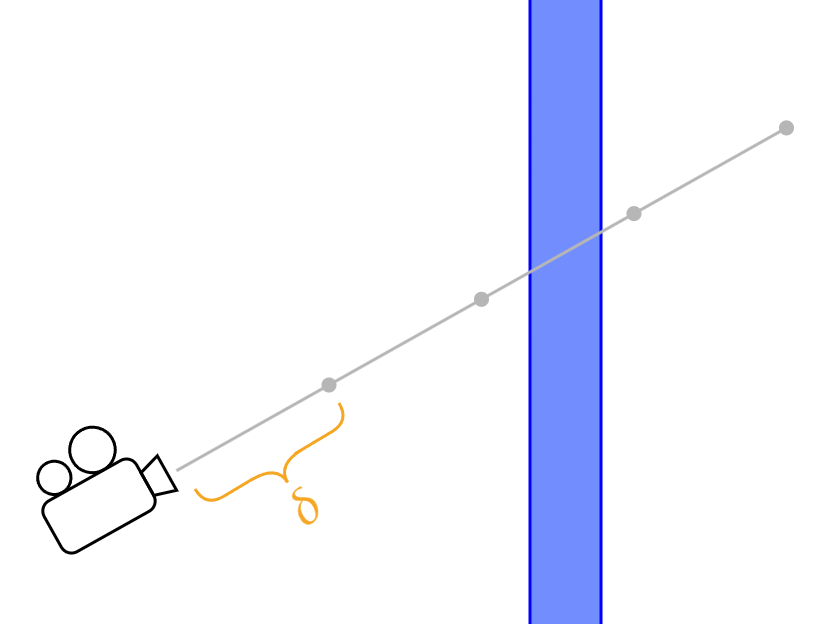
\includegraphics[width=0.4\textwidth]{Plantilla-TFG-master/img/miss.png}
    \caption{Pérdida de intersección en \textit{raymarching} para valores elevados de $\delta$}
    \label{fig:missInter}
\end{figure}

\SetKwComment{Comment}{// }{}
\begin{figure}[ht!]
    \centering
    \begin{minipage}{0.58\textwidth}
        \begin{algorithm}[H]
            \caption{Raymarching}
                \KwData{origen del rayo $c_o$, dirección del rayo $v$}
                \KwResult{terna RGB con el color del píxel actual}
                
                $d \gets 0$ \Comment{distancia total}
                
                \For{i $\in$ MAX\_ITERACIONES} {
                    $p \gets c_o +d\cdot v$
                    
                    sdf $\gets \phi(\text{p})$
                    
                    \If{sdf $< \varepsilon$}{
                       \Return{DibujarSuperficie($p,v,sdf$)}
                    }
            
                    $d\gets d + \delta$\;
            
                    \If{$d >$ MAX\_DISTANCIA}{
                        \Return{DibujarFondo()}
                    }
                }
        \end{algorithm}
    \end{minipage}%
    \hfill
    \begin{minipage}{0.4\textwidth}
        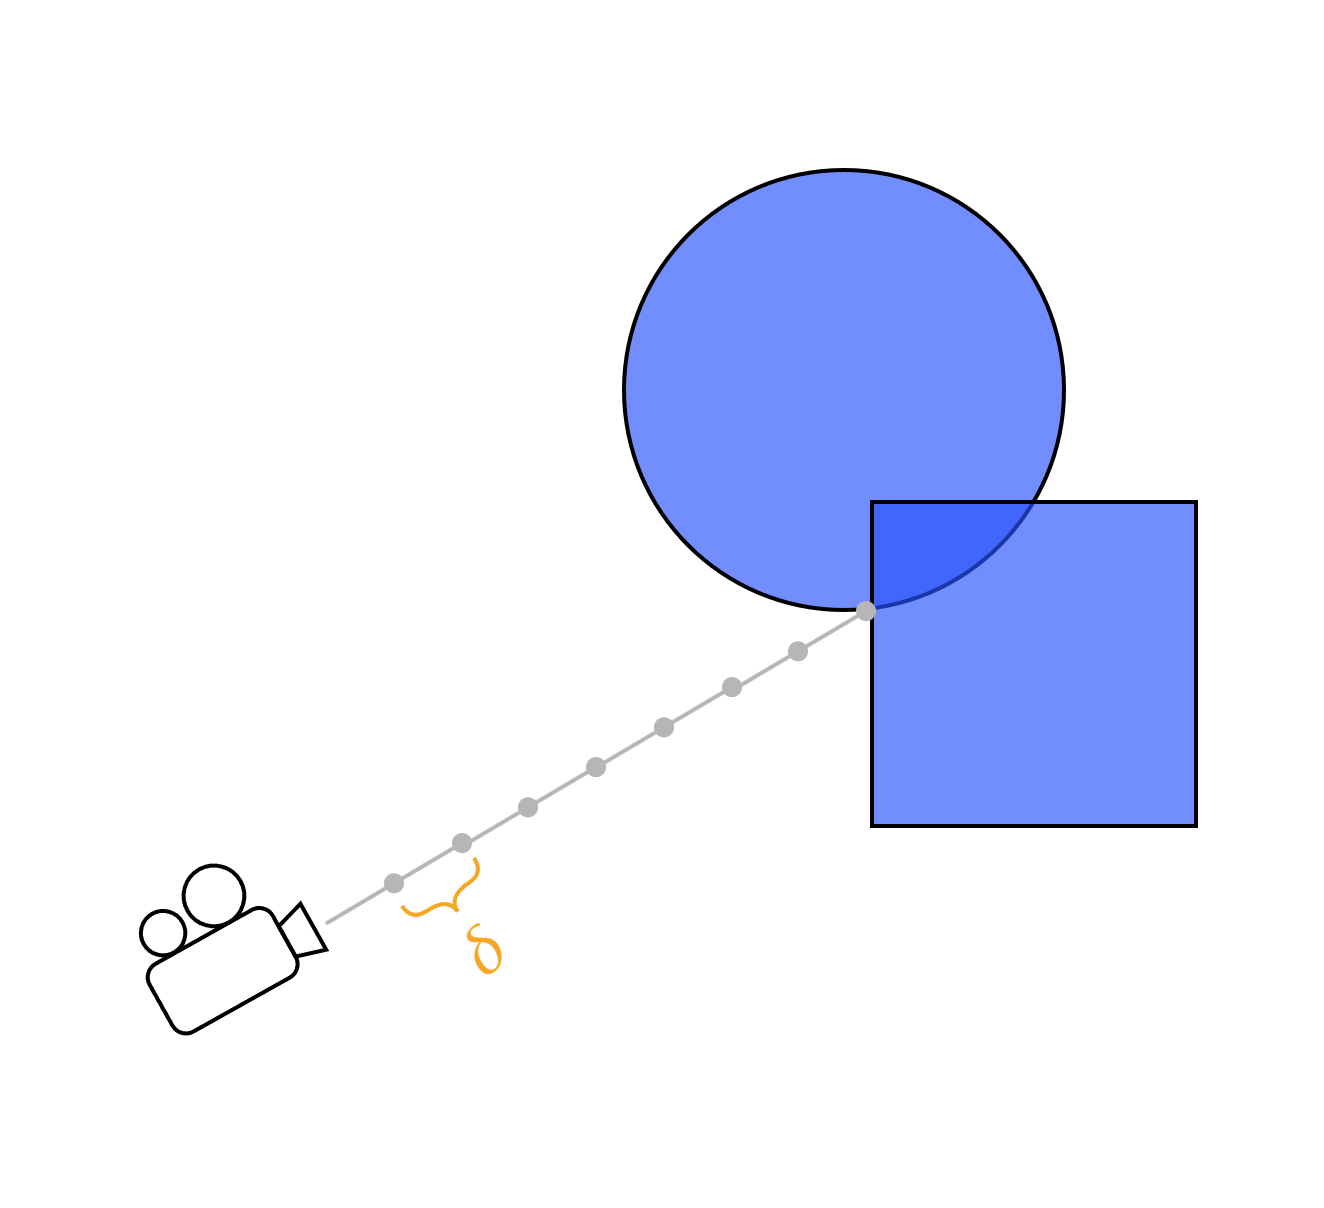
\includegraphics[width=\textwidth]{raymarching.png}
    \end{minipage}
    \caption{Algoritmo de \textit{raymarching}}
    \label{a:raymarching}
\end{figure}

Una desventaja de esta técnica es que puede ser bastante lenta, ya que cuanto más alejados estén los puntos de $S_\phi$ del observador, mayor es el número de iteraciones necesarias para encontrar la intersección en caso de que la haya. En el peor de los casos en el que tal intersección no exista, se habrá realizado el número máximo de iteraciones, que además será bastante alto debido a que el valor de incremento $\delta$ debe ser pequeño si no queremos perder ninguna intersección, como ocurre en la \autoref{fig:missInter}.\newline

Como solución a este problema aparece el \textit{spheretracing}, que reduce drásticamente el número de iteraciones, y por tanto de evaluaciones de $\phi$, necesarias para detectar la intersección. Su funcionamiento es similar al \textit{raymarching}, con la diferencia de que el incremento en la posición del rayo no es fija, sino que es la máxima que podemos tomar en cada momento asegurándonos de no perdernos una intersección. Esta distancia será la mínima del punto actual del rayo a $S_\phi$, que no es más que evaluar $\phi$ en dicho punto.\newline

Este será por tanto el algoritmo que utilizaremos para detectar qué pixels de la pantalla corresponden a la superficie $S_{\phi}$, y se encuentra descrito con detalle en la \autoref{a:spheretracing}. 
Con esto al fin podemos describir la forma que tendrá nuestro \textit{fragment shader} en la \autoref{fig:mainFS}. Claro está que esta versión todavía no es funcional, pues no sabemos qué forma tiene \texttt{DibujarSuperficie}, y como mucho podremos obtener una imagen que separe la isosuperficie del fondo usando colores planos como muestra la \autoref{fig:planos} para una esfera centrada en el origen. Veremos como mejorar esto en la próxima sección.

\begin{figure}[ht!]
    \centering
    \begin{minipage}{0.58\textwidth}
       \begin{algorithm}[H]
            \caption{Spheretracing}
                \KwData{origen del rayo $c_o$, dirección del rayo $v$}
                \KwResult{terna RGB con el color del píxel actual}
                $d \gets 0$ \Comment{distancia actual}
                
                \For{i $\in$ MAX\_ITERACIONES} {
                    $p \gets c_o + d \cdot v$
                    
                    $sdf \gets \phi(p)$
                    
                    \If{sdf $< \varepsilon$}{
                       \Return{$DibujarSuperficie(p,v,sdf)$}
                    }
            
                    $d \gets$ d + sdf
            
                    \If{$d >$ MAX\_DISTANCIA}{
                        \Return{$DibujarFondo()$}
                    }
                }
        \end{algorithm}
    \end{minipage}%
    \hfill
    \begin{minipage}{0.4\textwidth}
        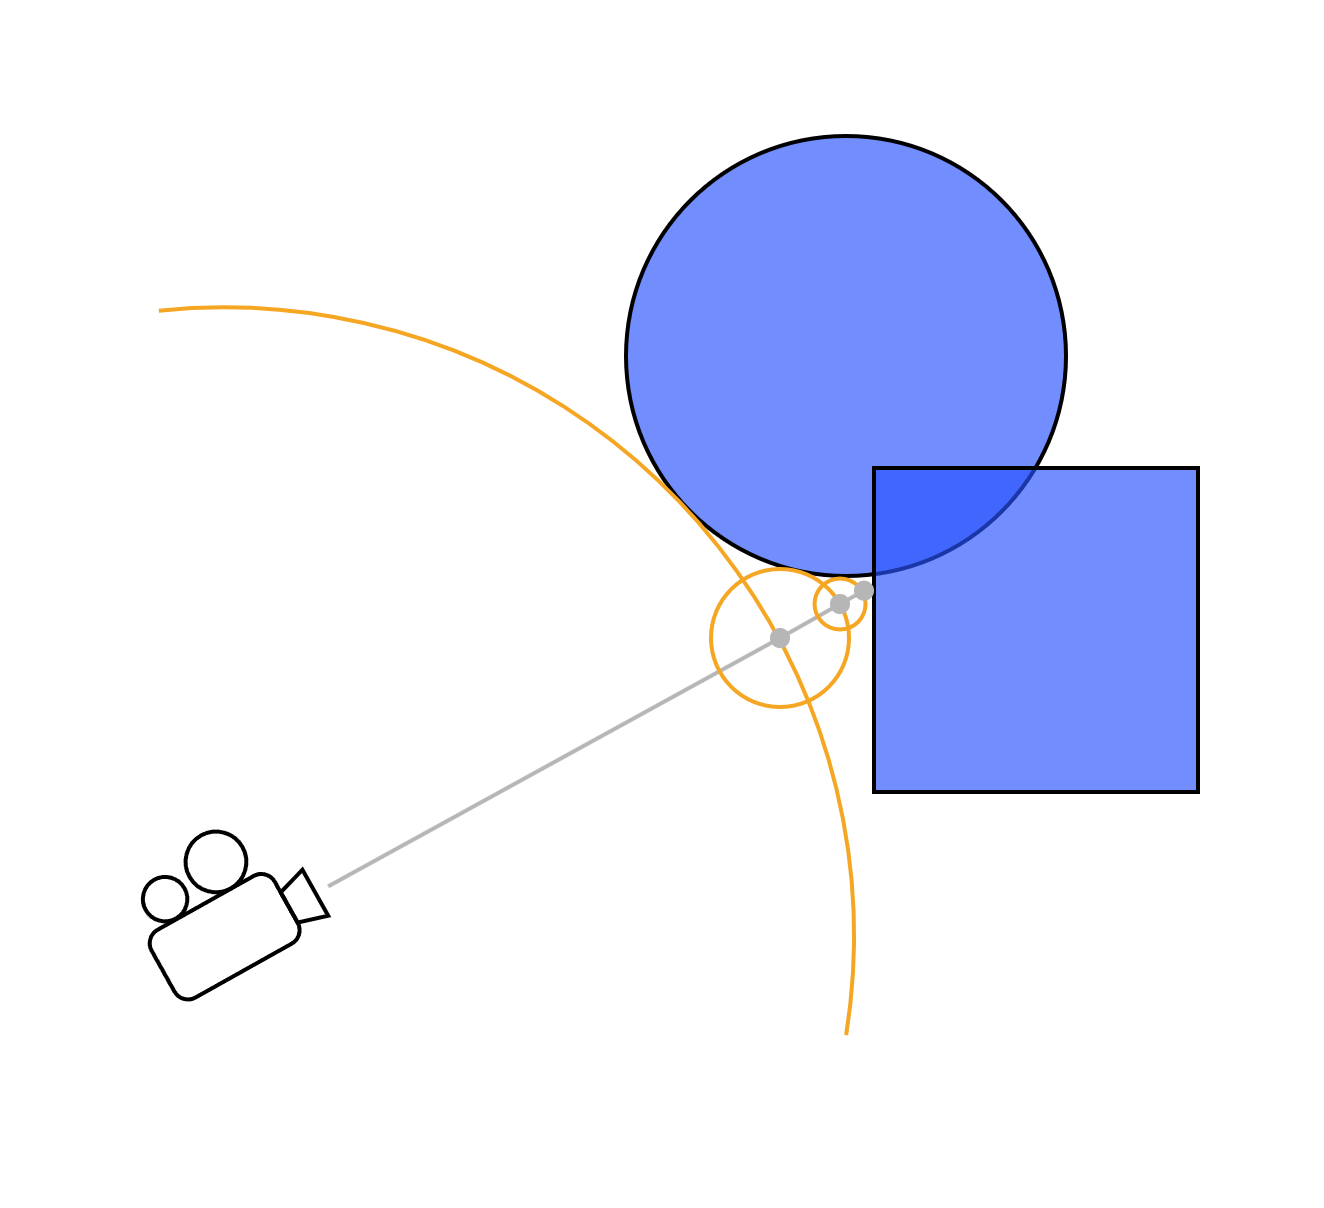
\includegraphics[width=\textwidth]{spheremarching.png}
    \end{minipage}
    \caption{Algoritmo de \textit{spheretracing}}
    \label{a:spheretracing}
\end{figure}

\begin{figure}[ht!]
    \centering
    
       \begin{algorithm}[H]
            \caption{Fragment Shader}
            \KwData{coordenadas de dispositivo $v_{frag}$ del píxel actual}
            \KwResult{color del píxel actual como terna RGBA $v_{col}$}

                $c_0 \gets $ posición de cámara en función de la entrada del ratón

                $l\gets $ punto de atención elegido por el usuario
                
                $uv \gets 2\cdot \frac{v_{frag} - 0.5\cdot u\_resolution}{u\_resolution_y}$\\[5pt]

                $f_1,\ f_2,\ f_3 \gets CalcularMarcoCartesiano(c_0, l)$
                
                $r_d \gets (f_1\ \vert \ f_2\ \vert \ f_3)\cdot normalizar ((uv_x, uv_y,-1))$\\[5pt]

                $color \gets$ spheretracing$(c_0, r_d)$\\[5pt]

                $v_{col} \gets (color_x, color_y, color_z, 1)$
        \end{algorithm}
    \caption{Cuerpo del método \texttt{main} del \textit{fragment shader}}
    \label{fig:mainFS}
\end{figure}


\begin{figure}[ht!]
    \centering
    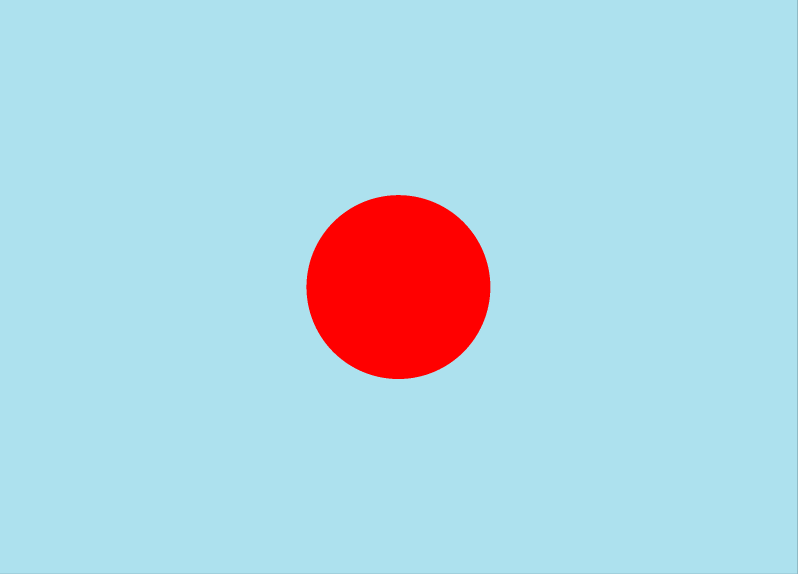
\includegraphics[width=0.8\textwidth]{Plantilla-TFG-master/img/escenaPlana.png}
    \caption{Resultado de \textit{spheretracing} asignando colores planos}
    \label{fig:planos}
\end{figure}


\section{Modelos de iluminación y sombras}\label{sec:ilum}
Ya sabemos qué pixels pertenecen a la superficie, pero no de qué color deben dibujarse. En esta sección estudiaremos diversas técnicas que en conjunto nos permitirán simular de forma plausible qué ocurre cuando se añaden a la escena una o varias fuentes de luz.


\subsection{Modelos de Blinn y Blinn-Phong}
Empezamos viendo cómo las fuentes de luz presentes en la escena iluminan directamente la superficie. Hay multitud de modelos que simulan este comportamiento de forma más o menos realista, siendo uno de los más extendidos el renderizado basado en física (\textit{physically based rendering} o PBR). Sin embargo, este y otros acercamientos similares son utilizados cuando se requiere de un alto grado de fidelidad y adaptabilidad. Nosotros usaremos el modelo de reflexión de Blinn-Phong \cite{apuntes:ig}, también popular pero mucho más simple y computacionalmente menos costoso. A su vez este modelo se basa en el de Blinn, el cual pasamos a estudiar a continuación. \newline

Vamos a considerar que nuestra escena consta de los siguientes elementos.
\begin{itemize}
    \item La \textbf{isosuperficie} $S_{\phi}$ como único objeto a ser dibujado (aunque el modelo es válido para cualquier número de objetos en escena).
    \item Un \textbf{observador} que se encuentra en la posición $c_o\in\R^3$ mirando a un punto $p\in \R^3$.
    \item Un número finito $n$ de \textbf{fuentes de luz}. Llamaremos $l_i$ con $i\in \{1,\dots, n\}$ a los vectores normalizados que apuntan desde $p$ a la posición de cada fuente.
\end{itemize}

Empecemos comprendiendo el fenómeno físico que tratamos de simular. La luz que generan las fuentes no es más que radiación electromagnética. De forma ideal, esta radiación se puede ver como un flujo en el espacio de partículas llamadas \textbf{fotones} que siguen trayectorias rectilíneas a la par que interaccionan con el entorno. Cada una de estas partículas tendrá una energía radiante única en función de su longitud de onda, que irá transfiriendo a aquellos objetos con los que interaccione.

\begin{definicion}[Radiancia]
    Dado un punto $p\in\R^3$, llamamos \textbf{radiancia} a la densidad de energía radiante por unidad de tiempo de los fotones que pasan por un entorno de $p$ en una determinada dirección $v\in\R^3$ con $\Vert v\Vert = 1$. La denotaremos $L(p,v)$, y será representada mediante una terna RGB no acotada. Podemos distinguir a su vez varios tipos de radiancia.
    \begin{itemize}
        \item \textbf{Radiancia emitida $\boldsymbol{L_E(p,v)}$:} radiancia que emite el propio objeto, también llamada emisividad. Normalmente es de intensidad baja y la consideraremos constante.
        \item \textbf{Radiancia incidente $\boldsymbol{L_{I}}(p,v)$:} radiancia que recibe el punto $p$ desde la dirección $v$. 
        \item \textbf{Radiancia reflejada $\boldsymbol{L_{R}}(p,v)$:} cantidad de la radiancia incidente en $p$ que se refleja en la dirección $v$. 
\end{itemize}
\end{definicion}

El objetivo del modelo será por tanto describir la radiancia que percibe el observador desde su posición en el punto $p$. Para ello, se llevan a cabo una serie de simplificaciones:
\begin{itemize}
    \item En un modelo físicamente correcto la luz reflejada en cada punto se dispersaría por el entorno, contribuyendo a la radiancia incidente en otros puntos de la escena. Sin embargo, nosotros no consideraremos la radiancia incidente que no provenga directamente de fuentes de luz. Incluso teniendo un solo objeto en escena como es nuestro caso este modelo es mejorable, pues el objeto puede reflejar radiancia sobre sí mismo. Por tanto, usaremos una radiancia ambiente constante $L_A$ para suplir esta iluminación indirecta.
    \item La radiancia se conserva en el espacio entre objetos.
    \item Las fuentes de luz son direccionales, de forma que no serán visibles en la escena. Además supondremos que emiten una radiancia constante $S_i$ para $i\in \{1,\dots, n\}$.
    \item No se consideran objetos con transparencia.
\end{itemize}
Es natural pensar que la radiancia percibida en un punto $p\in \R^3$ será la suma de la radiancia que emita y la que sea capaz de reflejar. Así, teniendo en cuenta las consideraciones anteriores tenemos que
\begin{equation*}
    L(p,v) = L_A + L_E + \sum_{i=1}^n L_R(p,l_i).
\end{equation*}
Como $L_A$ y $L_E$ son constantes solo nos falta estudiar cómo obtener la \textbf{radiancia reflejada} para cada fuente de luz. Para ello fijamos un índice $m\in \{1,\dots,n\}$ y suponemos a partir de ahora que $p\in S_{\phi}$, pues de lo contrario

\begin{equation*}
    L(p,v) = L_A,\ p\in \R^3\setminus S_{\phi},
\end{equation*}
ya que la única luz que se puede reflejar es la del ambiente y ya está siendo considerada con $L_A$, y al trabajar únicamente con fuentes de luz direccionales $L_E=0$. \newline

Sabemos que cada objeto refleja la luz de manera distinta en función de su material y las propiedades de la fuente. Para representar este comportamiento definimos una función que indique la fracción de radiancia proveniente de $l_m$ que se refleja en un punto $p$ en la dirección $v$ para cada fuente de luz
\begin{equation*}
    f_r \colon \R^3\times \R^3\times \R^3 \to \R^3.
\end{equation*}
Así, la radiancia reflejada es
\begin{equation*}
    L_R(p,v,l_m) = S_m\cdot f_r(p,v,l_m).
\end{equation*}

Podemos distinguir diferentes tipos de reflexión, cada uno contribuyendo de forma diferente a la radiancia reflejada final.

% donde $f_a$, $f_d$ y $f_e$ representan la fracción de radiancia reflejada para cada uno de los tipos de reflexión que podemos distinguir y listamos a continuación. 
\begin{itemize}
    \item \textbf{Reflexión ambiental:} cantidad de iluminación indirecta proveniente de la fuente de luz que refleja el objeto. Al igual que hicimos con $L_A$, tomaremos un valor constante $R_A$ para ella, de forma que la fracción de radiancia ambiental reflejada será
    \begin{equation*}
        f_{ra} =  R_A \in \R^3.
    \end{equation*}
    \item \textbf{Reflexión especular:} define cómo se refleja la luz en objetos brillantes teniendo en cuenta la posición de la fuente de luz y la del observador. Según la ley de refracción, el ángulo de incidencia de la luz será igual al de reflexión, luego podemos obtener la dirección de reflexión $r_m$ reflejando $l_m$ sobre el vector normal unitario en $p$ de la superficie, que llamaremos $N_p$. Así,
    
    \begin{equation*}
        r_m = 2(l_m\cdot N_p)N_p - l_m \in \R^3.
    \end{equation*}

    Sin embargo, solo queremos que haya reflejos en los puntos orientados hacia la fuente de luz y cuando $r_m$ haya sido reflejado en una dirección que el observador pueda apreciar, siendo la intensidad del reflejo mayor cuanto más alineado esté el observador con el vector reflejado. Esto equivale a que se cumpla
    \begin{equation*}
        N_p\cdot l_m >0 \quad \text{ y }\quad  R_m \cdot v>0.
    \end{equation*}
    Para controlar el color y la intensidad de los reflejos usaremos una radiancia $R_E$, de forma que podemos expresar la fracción de radiancia especular reflejada como
    \begin{align*}
        f_{re} \colon \R^3\times \R^3\times \R^3 &\to \R^3,\\
        (p,v,l_m) &\mapsto R_E \cdot \Max(0,l_m\cdot N_p) \cdot \Max(0,r_m \cdot v).
    \end{align*}
    \item \textbf{Reflexión difusa:} modela cómo se refleja la luz en objetos mates en función de la posición de la fuente de luz. Al contrario de lo que ocurre con la reflexión especular, debido a la irregularidad de la superficie del objeto la luz no se refleja en una sola dirección, haciendo que se disperse en direcciones impredecibles. Este comportamiento se simula a través de una radiancia $R_D$ que represente el valor promedio resultado de estos reflejos, y que consideraremos constante. Al igual que antes, solo queremos que el punto esté iluminado cuando esté de cara a la fuente de luz, obteniendo la mayor cantidad de luz cuando está alineado con la fuente. Así, la fracción de radiancia difusa será
    \begin{align*}
        f_{rd} \colon \R^3\times \R^3\times \R^3 &\to \R^3,\\
        (p,v,l_m) &\mapsto R_D\cdot \Max(0,l_m \cdot N_p).
    \end{align*}
\end{itemize}

\begin{figure}[ht!]
    \centering
    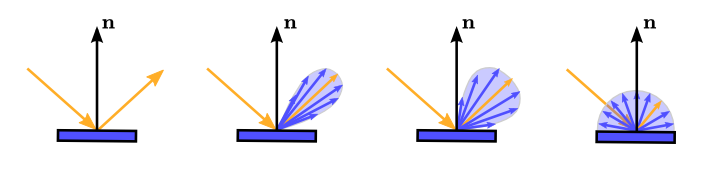
\includegraphics[width=0.85\textwidth]{Plantilla-TFG-master/img/glossyTodiffuse.png}
    \caption{Reflexión de un rayo en una superficie progresivamente más mate \cite{especular}}
    \label{fig:miss}
\end{figure}

\begin{observacion}
    Es necesario que los vectores $l_i$, $v$ y $N_p$ sean unitarios, pues de lo contrario su producto escalar no coincidiría con el coseno del ángulo que forman.
\end{observacion}

En vista de las definiciones anteriores, podríamos simplemente definir
\begin{equation*}
    f_r(p,v,l_m) = f_{ra}+f_{re}(p,v,l_m) + f_{r_d}(p,v,l_m).
\end{equation*}

De esta forma, para diferenciar entre un material totalmente mate como el yeso y uno especular como el metal bastaría tomar valores de $R_D$ y $R_E$ tal que $\Vert R_D\Vert \gg \Vert R_E\Vert$. Sin embargo, a la hora de comparar materiales especulares podríamos observar que aunque ambos generen zonas brillantes no lo hagan de la misma forma. Por ejemplo, tanto el mármol como el metal generan brillos sobre su superficie, pero en el caso del metal estos son más pequeños y brillantes debido a que se trata de un material más pulido. Por tanto, para añadir control sobre el tamaño e intensidad de estas zonas brillantes introducimos el \textbf{coeficiente de brillo} $\alpha \in \R$ en la expresión de $f_{re}$, de forma que cuanto mayor sea su valor más pequeños e intensos serán los brillos generados. En la \autoref{fig:parametrosEspecular} podemos ver el efecto que tienen $R_E,R_D$ sobre la radiancia reflejada \cite{especular}.\newline

\begin{definicion}
    Dado un objeto, definimos su \textbf{material} como la tupla $\{R_A,R_E,R_D,\alpha \}$.
\end{definicion}

Una vez asociado un material a $S_{\phi}$ podemos escribir la expresión final para $f_r$:

\begin{align}\label{eq:fr}
    f_r(p,v,l_i) &= f_{ra} &+\ & f_{re}(p,v,l_i) &+\ &f_{r_d}(p,v,l_i)\\
                 &= R_A    &+\ & R_E \cdot \Max(0,l_i\cdot N_p) \cdot \Max(0,r_i \cdot v)^{\alpha} &+\  &R_D\cdot \Max(0,l_i\cdot N_p). 
\end{align}

\begin{figure}[!h]
     \begin{minipage}[c]{0.45\linewidth}
        \centering
        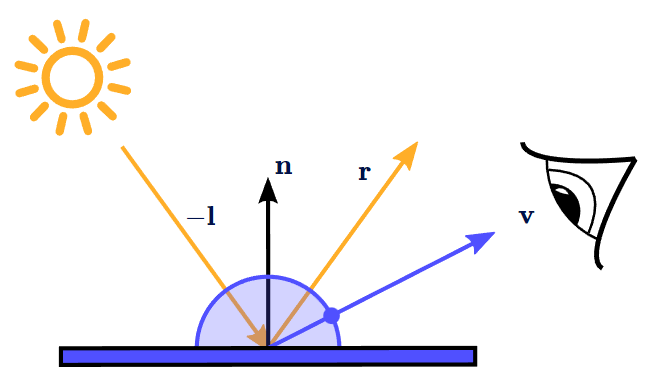
\includegraphics[width=0.95\textwidth]{Plantilla-TFG-master/img/ks0kd1.png}
        \caption{$\Vert R_E\Vert = 0$}
     \end{minipage}
     \begin{minipage}[c]{0.45\linewidth}
        \centering
        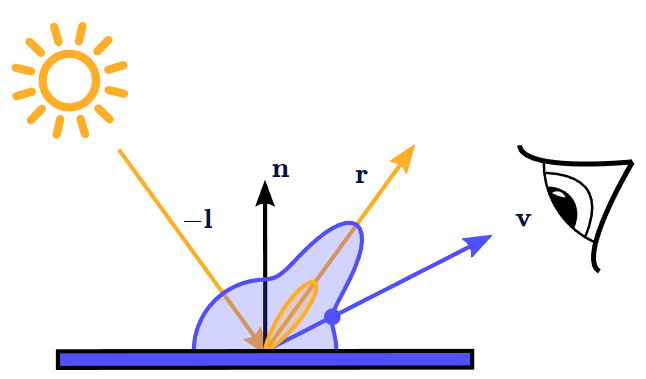
\includegraphics[width=0.95\textwidth]{Plantilla-TFG-master/img/ks1kd1.png}
        \caption{$\Vert R_E\Vert =\Vert R_D\Vert$ y $\alpha$ grande}
     \end{minipage}
     \begin{minipage}[c]{0.45\linewidth}
        \centering
        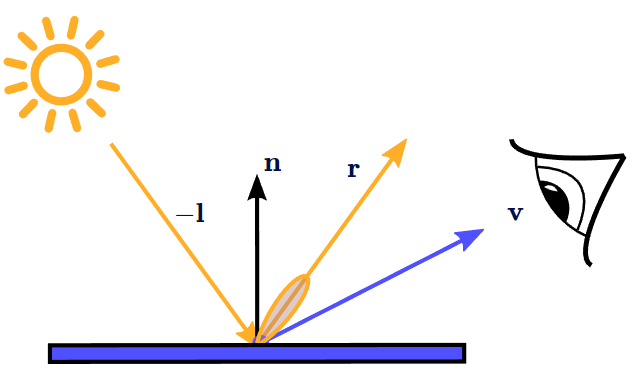
\includegraphics[width=0.95\textwidth]{Plantilla-TFG-master/img/ks1kd0.png}
        \caption{$\Vert R_D\Vert = 0$}
     \end{minipage}
     \begin{minipage}[c]{0.45\linewidth}
        \centering
        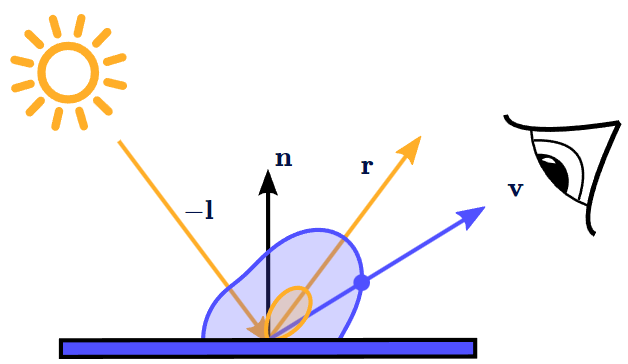
\includegraphics[width=0.95\textwidth]{Plantilla-TFG-master/img/ks1kd1a0.png}
        \caption{$\Vert R_E\Vert =\Vert R_D\Vert$ y $\alpha$ pequeño}
     \end{minipage}
     % \begin{minipage}[c]{0.45\linewidth}
     %    \centering
     %    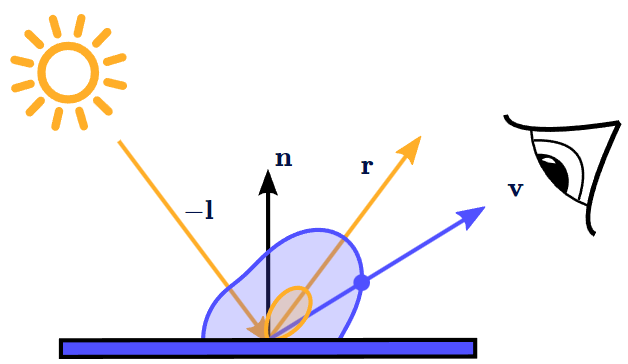
\includegraphics[width=0.95\textwidth]{Plantilla-TFG-master/img/ks1kd1a0.png}
     %    \caption{$k_s = 1$ y $k_d = 0$}
     % \end{minipage}
     \caption{Ejemplo de distintos valores para $R_E,R_D$ y $\alpha$}
     \label{fig:parametrosEspecular}
\end{figure}

Recogemos los resultados obtenidos en la siguiente definición.
\begin{definicion}[Modelo de Blinn]\label{def:blinn} La radiancia percibida en el punto $p\in\R^3$ desde la dirección $v\in\R^3$ con $\Vert v\Vert = 1$ según el modelo de Blinn viene dada por
    \begin{equation*}
        L(p,v) = L_A+L_E+ \sum_{i=0}^n S_i \Bigg[ k_aR_A + \Max(0,l_i\cdot N_p) \Big( k_dR_D + k_eR_E\cdot \Max(0,r_i\cdot v) \Big) \Bigg],
    \end{equation*}

    donde:
    \begin{itemize}
        \item $n \in \N$ es el número de fuentes de luz y $l_i \in R^3$ es el vector normalizado que apunta a $p$ desde cada una de ellas,
        \item $L_A,L_E \in \R^3$ son ternas RGB no acotadas representando la radiancia ambiente y emitida respectivamente,
        \item $S_i \in \R^3$ es una terna RGB no acotada representando la radiancia emitida por la fuente de luz $i$-ésima,
        \item $\alpha \in \R$ es el coeficiente de brillo,
        \item $R_A,R_D,R_E \in \R^3$ son ternas RGB (no acotadas) representando la radiancia reflejada de forma ambiental, difusa y especular respectivamente,
        \item $N_p$ es el vector normal de la superficie en $p$ y $r_i$ es el vector $l_i$ reflejado sobre $N_p$.
    \end{itemize}
\end{definicion}

En 1975 Phong \cite{phong} introdujo una variante a este modelo que hoy conocemos como \textbf{modelo de Blinn-Phong}. Su única diferencia con el de Blinn consiste en el uso del llamado \textit{halfway vector}
\begin{equation*}
    h_m = \frac{l_m + v}{\Vert l_m + v\Vert}.
\end{equation*}

Ahora, en lugar de usar el valor $r_m\cdot v$ hacemos que el brillo sea proporcional al coseno del ángulo entre $h_m$ y $N_p$, de forma que no depende del punto $p$ y solo necesita ser calculado una vez. En la \autoref{fig:phong} podemos ver el comportamiento de $h_m$ para distintas configuraciones de $l_m$ y $v$.
\begin{figure}[!h]
     \begin{minipage}[c]{0.32\linewidth}
        \centering
        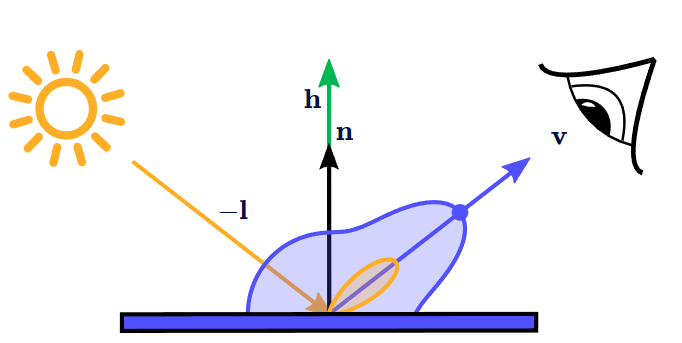
\includegraphics[width=0.95\textwidth, align=b]{Plantilla-TFG-master/img/phong1.png}
     \end{minipage}
     \begin{minipage}[c]{0.32\linewidth}
        \centering
        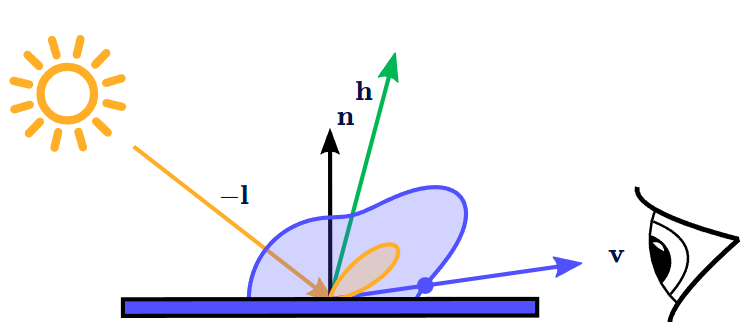
\includegraphics[width=0.95\textwidth, align=b]{Plantilla-TFG-master/img/phong2.png}
     \end{minipage}
     \begin{minipage}[c]{0.32\linewidth}
        \centering
        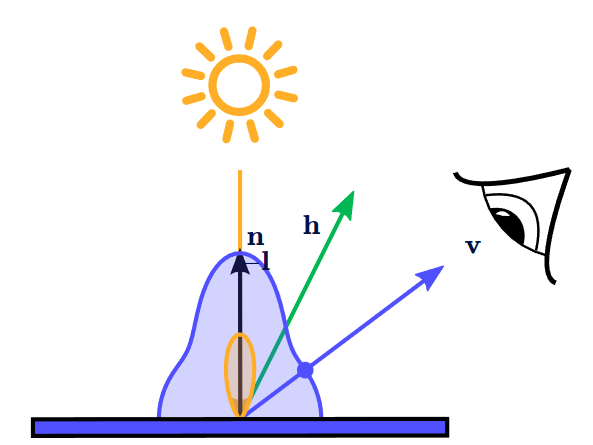
\includegraphics[width=0.95\textwidth, align=b]{Plantilla-TFG-master/img/phong3.png}
     \end{minipage}
     \caption{Comportamiento de  $h_m$ con $\Vert R_S\Vert =\Vert R_D\Vert$}
     \label{fig:phong}
\end{figure}

Aunque pueda parecer una simplificación del modelo de Blinn, lo cierto es que produce resultados más convincentes que este. En particular, mientras que el modelo de Blinn siempre produce brillos redondos en superficies planas, el de Blinn-Phong los genera con una forma más elíptica cuando se observa la superficie desde un ángulo acusado, como se observa en la \autoref{fig:difBlinn}. 

\begin{figure}[!h]
     \begin{minipage}[c]{0.49\linewidth}
        \centering
        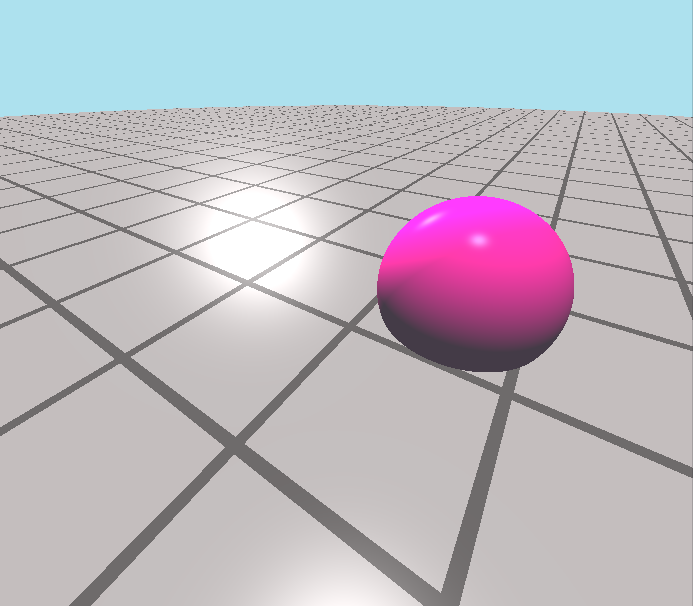
\includegraphics[width=0.9\textwidth]{Plantilla-TFG-master/img/compB.png}
        \caption{Blinn}
     \end{minipage}
     \begin{minipage}[c]{0.49\linewidth}
        \centering
        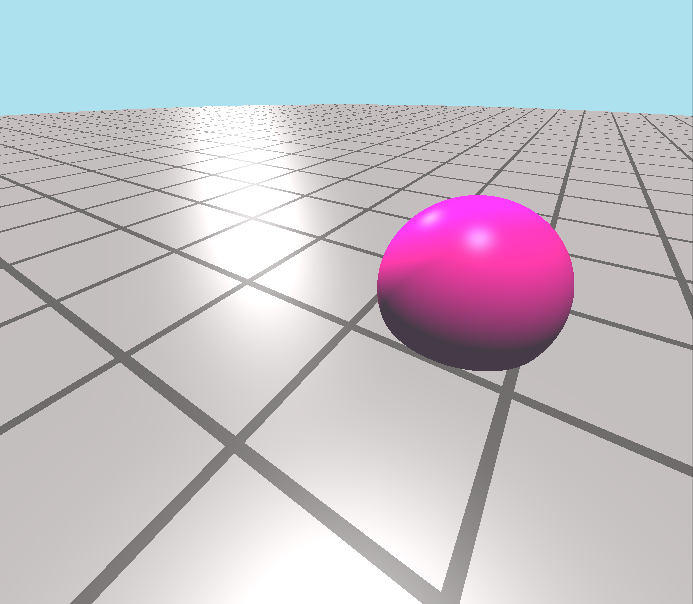
\includegraphics[width=0.9\textwidth]{Plantilla-TFG-master/img/compBP.png}
        \caption{Blinn-Phong}
     \end{minipage}
     \caption{Zonas brillantes en modelos de Blinn y Blinn-Phong}
     \label{fig:difBlinn}
\end{figure}

\begin{definicion}[Modelo de Blinn-Phong]
    En el contexto de la \autoref{def:blinn}, la radiancia percibida en el punto $p\in\R^3$ desde la dirección $v\in\R^3$ con $\Vert v \Vert = 1$ según el modelo de Blinn-Phong viene dada por
    \begin{equation*}
        L(p,v) = L_A+L_E+ \sum_{i=0}^n S_i \Bigg[ k_aR_A + \Max(0,l_i\cdot N_p) \left( k_dR_D + k_eR_E\cdot \left(N_p\cdot \frac{l_i + v}{\Vert l_i + v\Vert} \right)^{\alpha} \right) \Bigg].
    \end{equation*}
\end{definicion}

Ya podemos darle forma a las funciones \texttt{DibujarSuperficie} y \texttt{DibujarFondo} usadas en la \autoref{a:spheretracing}, suponiendo que pasamos como \textit{uniforms} los parámetros del material y los valores $l_i$ y $S_i$ para cada $i\in \{1,\dots, n\}$.
\begin{figure}[ht!]
    \centering
    
       \begin{algorithm}[H]
            \caption{DibujarSupercicie}
                \KwData{punto $p$, dirección del rayo $v$, distancia $\phi(p)$}
                \KwResult{terna RGB con la radiancia percibida en el punto $p$}
                $L \gets L_A$ \Comment{Radiancia final}
                \For{$i \in \{1,\dots, n\}$} {

                    
                    $h \gets normalizar(L_i - v)$ \Comment{Observador en dirección opuesta a la del rayo}
                    
                    $N_p \gets$ CalcularNormal$(p)$
                    
                    $NLi \gets \Max(0,\ N_p\cdot l_i)$
                    
                    $NH \gets \Max(0,\ N_p \cdot h)$\newline

                    $f_{ra} = R_A$
                    
                    $f_{rd} = NLi\cdot R_D$
                    
                    $f_{re} = NLi \cdot R_E \cdot NH^{\alpha}$\newline

                    $L \gets L + S_i\cdot (f_{ra} + f_{rd} + f_{re})$
                }

                \Return{$L$}
        \end{algorithm}
    \begin{algorithm}[H]
            \caption{DibujarFondo}
                \KwResult{terna RGB con el color de fondo de la escena}
                \Return{$L_A$}
        \end{algorithm}

        \caption{Implementación de las funciones \texttt{DibujarSuperficie} y \texttt{DibujarFondo}}
\end{figure}

Solo queda un asunto por tratar. A la vista de la expresión de $f_r$ \eqref{eq:fr} y del código anterior, somos capaces de calcular todos los valores a excepción de uno, el del vector normal. En la siguiente sección veremos presentamos una técnica para calcularlo de forma aproximada. 

\subsubsection{Cálculo del vector normal}
En cualquier modelo de iluminación el acceso al vector normal es indispensable. Cuando se trabaja con mallas de polígonos el vector normal viene dado para cada vértice, pero este no es nuestro caso. En su lugar nosotros usaremos el gradiente de la función distancia con signo para obtenerlo \cite{harvard}.
\begin{proposicion}\label{p:gradient_perp}
  Sea $\phi\colon \R^3\to \R$ diferenciable. Entonces $\nabla\phi$ es perpendicular a $S_\phi$.
\end{proposicion}
\begin{proof}
  Sea $s\in S_\phi$ arbitrario. Tomamos una curva parametrizada:
  \begin{align*}
    \alpha \colon [0,1] & \to S_\phi,\\
    t                   & \mapsto \left(x(t), y(t), z(t) \right),
  \end{align*}
  cumpliendo $\alpha(t_0)=s$ para algún $t_0\in [0,1]$. Veamos que $\nabla\phi(s) \perp \alpha$. Como $ \alpha(t)\subset S_\phi$ la evaluación de $\phi$ en cualquier punto de la curva será cero, y por tanto
  \begin{equation*}
      \frac{d}{dt}\phi(\alpha(t)) = 0.
  \end{equation*}
  Aplicando la regla de la cadena obtenemos
  \begin{equation*}
       \frac{d\phi \circ \alpha}{dt} = \frac{\partial{\phi}}{\partial{x}}\bigg\rvert_s \frac{dx}{dt}\bigg\rvert_{t_0} + \frac{\partial{\phi}}{\partial{y}}\bigg\rvert_s\frac{dy}{dt}\bigg\rvert_{t_0} + \frac{\partial{\phi}}{\partial{z}}\bigg\rvert_s\frac{dz}{dt}\bigg\rvert_{t_0} = \nabla \phi (s) \cdot \frac{d\alpha}{dt}\bigg\rvert_{t_0} = 0.
  \end{equation*}
    Por tanto $\nabla\phi(s)$ es perpendicular al vector tangente de $\alpha$ en $s$, que a su vez está contenido en el plano tangente de $S_\phi$ en $s$, luego $\nabla\phi(s) \perp S_\phi$.
\end{proof}

Hemos visto que calcular el vector normal en cualquier punto equivale a calcular $\nabla\phi$ y que este existe en casi todo punto de $S_{\phi}$ por el \autoref{teo:diff}, pero esto no significa que podamos o debamos obtenerlo de forma analítica. Si bien en muchos casos sería posible hacerlo de forma analítica, esto podría tener asociado un coste computacional que no podemos asumir. Existen varios métodos numéricos para aproximar el gradiente de una función. Uno de los más triviales es el de las diferencias centrales, basado en aproximar el límite de la \autoref{def:parcial} tomando un valor pequeño para $h$. Necesitaríamos entonces realizar seis evaluaciones de $\phi$ para obtener el gradiente, dos por cada parcial. Nosotros usaremos el \textbf{método del tetraedro} \cite{article:tetra}, que sin ser el más preciso,  produce buenos resultados y es rápido, haciendo uso únicamente de cuatro evaluaciones de $\phi$ en la dirección de los vértices de un tetraedro:


\begin{equation*}
    k_0 = (1,-1,-1),\quad k_1 = (-1,-1,1),\quad k_2=(-1,1,-1),\quad k_3=(1,1,1).
\end{equation*}

\begin{proposicion}[Método del tetraedro]
  Dado $p\in S_\phi$, una aproximación de su vector normal $N_p$ se obtiene normalizando el vector
  \begin{equation*}
    \hat{N_p} = \sum_{i=0}^3 k_i\cdot f(p + hk_i)\quad \text{, donde } h\approx 0.
  \end{equation*}
\end{proposicion}

\begin{proof}
  Por la proposición \autoref{p:gradient_perp}, basta comprobar que $\hat{N}$ es colineal a $\nabla \phi(p)$.
  \begin{align*}
    \hat{N} & = \sum_{i=0}^3 k_i\cdot f(p + hk_i) = \sum_{i=0}^3 k_i\cdot f(p + hk_i) - k_i\cdot f(p) = \sum_{i=0}^3 k_i\cdot \left[ f(p+hk_i) - f(p)\right]\\ &= h\sum_{i=0}^3 k_i \nabla_{k_i}f(x)
    = h\sum_{i=0}^3 k_i \cdot \left( k_i \cdot \nabla f(p)\right) = h\sum_{i=0}^3 (k_i\cdot k_i) \nabla f(p) = h\sum_{i=0}^3 \nabla f(p) = 4h\nabla f(p).
  \end{align*}
  Hemos usado que $\sum_{i=0}^3 k_i = (0,0,0)$, $\sum_{i=0}^3 k_i\cdot k_i = (1,1,1)$ y que el producto escalar es un operador lineal.
\end{proof}

\subsection{Sombras}
Los resultados obtenidos en la \autoref{fig:difBlinn} presentan ciertas carencias, siendo la más flagrante la ausencia de sombras arrojadas, que no son consideradas en el modelo de Blinn-Phong. Afortunadamente el uso de las SDFs nos hará la obtención de la información necesaria para añadir sombras a nuestra escena muy sencilla. Para saber si un punto $p\in\R^3$ recibe luz de una $i$-ésima fuente de luz bastará comprobar si hay algún obstáculo entre dicha fuente y el punto. Para hacer esta comprobación usaremos de nuevo \textit{spheretracing}, pero en esta ocasión desde el punto hacia la fuente de luz. Si se detecta alguna intersección significará que el punto $p$ no recibe luz de la fuente y por tanto $L_R(p,v,l_i) = 0,\ \forall v\in \R^3$. Podemos modificar \texttt{DibujarSuperficie} como se muestra en la \autoref{fig:sombras1} para añadir este comprobación.\newline

\begin{algorithm}[H]
        \caption{DibujarSupercicie}
            \KwData{punto $p$, dirección del rayo $v$, distancia $\phi(p)$}
            \KwResult{terna RGB con la radiancia percibida en el punto $p$}
            $L \gets L_A + L_E$ \Comment{Radiancia final}
            \For{$i \in \{1,\dots, n\}$} {

                \Comment{ ··· }
                $sombras \gets CalcularSombras(p, l_i)$

                $L \gets L + S_i\cdot (f_{ra} + f_{rd} + f_{re})\cdot sombras$
            }

            \Return{$L$}
    \end{algorithm}
\begin{figure}[ht!]
    \centering
    \begin{minipage}{0.50\textwidth}
   \begin{algorithm}[H]
            \caption{CalcularSombras}
                \KwData{punto $p_0$, dirección de luz $l_i$}
                \KwResult{factor de sombra en $p_0$ en el rango $[0,1]$}
                 $d \gets \delta$ \Comment{distancia actual}
                
                \For{i $\in$ MAX\_ITERACIONES} {
                    $p \gets p_o + d \cdot v$
                    
                    $sdf \gets \phi(p)$
                    
                    \If{sdf $< \varepsilon$}{
                       \Return{0};
                    }
            
                    $d \gets d + sdf$

                    \If{d > MAX\_DISTANCIA}{
                        \Return{1}
                    }
                }

                \Return{1}
        \end{algorithm}
    \end{minipage}%
    \hfill
    \begin{minipage}{0.48\textwidth}
        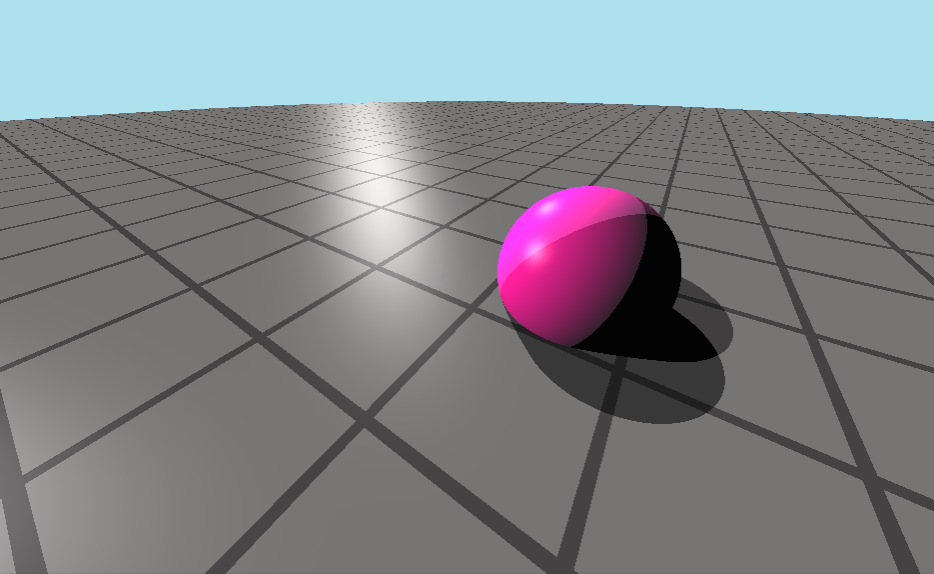
\includegraphics[width=\textwidth]{shadowSimple.png}
    \end{minipage}
    \caption{Cálculo básico de sombras}
    \label{fig:sombras1}
\end{figure}


Realizamos las siguientes apreciaciones respecto al método \texttt{CalcularSombras} propuesto:
\begin{itemize}
    \item Dado que estamos trabajando con luces direccionales situadas a distancia infinita solo podemos hacer \textit{spheretracing} desde $p$ en dirección a la fuente, a pesar de que lo intuitivo sería hacerlo desde el foco de luz hacia el punto.
    \item A diferencia del algoritmo propuesto en \autoref{a:spheretracing} no podemos inicializar $d=0$, ya que entonces se detectaría una intersección en el mismo punto $p$.
\end{itemize}

Estudiando los resultados obtenidos vemos que al añadir sombras obtenemos una imagen mucho más cohesiva y otorgamos a la esfera mayor presencia en la escena. Sin embargo también podremos apreciar que las sombras que genera este método son muy planas y duras. Realmente ahora mismo no tenemos control alguno sobre esto, ya que según nuestra implementación un punto o está totalmente en sombra o totalmente iluminado. Esto no siempre es así en el mundo real, donde podemos encontrar que no toda la región sombreada sea igual de oscura o el borde esté más o menos difuminado en función de las propiedades de la fuente. Podemos simular estos fenómenos de forma muy sencilla usando información de la que ya que disponemos en el algoritmo de \textit{spheretracing}. En particular:
\begin{itemize}
    \item Haremos que cuanto más cerca se encuentre el punto del obstáculo que le hace sombra menos luz reciba. Por tanto la intensidad de la sombra será proporcional a la evaluación de la SDF en el punto actual del rayo:
    \begin{equation*}
        sombra \propto sdf.
    \end{equation*}
    \item Cuando un punto sea alcanzado por la luz pero haya estado muy cerca de ser obstruido dejaremos que refleje solo una fracción de la luz total. Esta cantidad deberá ser mayor cuanto menos haya faltado para perder la intersección, creando un difuminado en el borde:
    \begin{equation*}
        sombra \propto \frac{1}{d}.
    \end{equation*}
\end{itemize}

Esta nueva versión de \texttt{CalcularSombras} se encuentra descrita en la \autoref{fig:sombras2}. En ella se ha añadido un parámetro $k\in \R_0^+$ para controlar la intensidad del efecto de suavizado. En realidad este parámetro hace referencia al \textbf{tamaño de la fuente de luz}, en concreto a su inversa. Así, cuanto más pequeño sea este valor más grande será la fuente de luz, produciendo sombras más difusas. Por ejemplo, el Sol tendrá un valor pequeño para $k$, mientras que una bombilla lo tendría grande. A partir de ahora en nuestra escena de ejemplo fijamos $k=  1.5$ para la fuente de luz que apunta más hacia la cámara, que actuará como el Sol, y $k = 10$ para la otra, que actuará como una linterna.\newline

\begin{figure}[ht!]
    \centering
    \begin{minipage}{0.50\textwidth}
       \begin{algorithm}[H]
            \caption{CalcularSombras}
                \KwData{punto $p_0$, dirección de luz $l_i$, tamaño de luz $k$}
                \KwResult{factor de sombra en $p_0$ en el rango $[0,1]$}
                $sombra \gets 1$
                
                $d \gets \delta$ \Comment{distancia actual}
                
                \For{i $\in$ MAX\_ITERACIONES} {
                    $p \gets p_o + d \cdot v$
                    
                    $sdf \gets \phi(p)$
                    
                    \If{sdf $< \varepsilon$}{
                       \Return{0};
                    }
                    $sombra \gets \Min(sombra, k\cdot \frac{sdf}{d})$
                    
                    $d \gets d + sdf$

                    \If{d > MAX\_DISTANCIA}{
                        \Return{1}
                    }
                }

                \Return{1}
        \end{algorithm}
    \end{minipage}%
    \hfill
    \begin{minipage}{0.48\textwidth}
        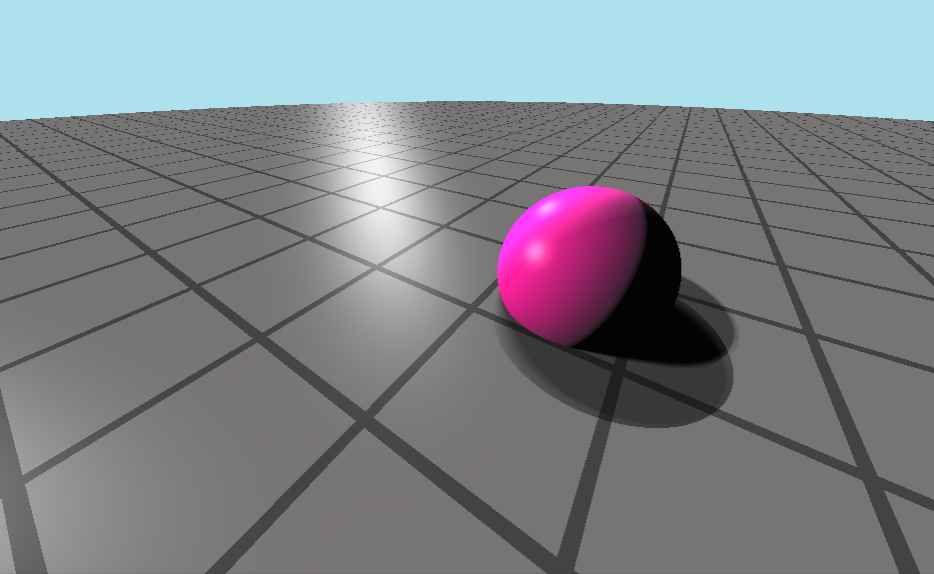
\includegraphics[width=\textwidth]{shadowSoftArtifact.png}
    \end{minipage}
    \caption{Cálculo de sombras suavizadas}
    \label{fig:sombras2}
\end{figure}

Si bien este método genera resultados más realistas en general, también puede generar ciertas imperfecciones en el borde de la sombra, como se puede apreciar en la \autoref{fig:artifactZoom}. Esto es debido a que en el proceso de \textit{spheretracing} podemos saltarnos una intersección que habría aportado más oscuridad que la que finalmente se ha encontrado, generando fugas de luz que siguen el patrón de los puntos en los que se evalúa la SDF. Hay varias formas de solventar esto, como la propuesta por Sebastian Aaltonen \cite{gdc} en la GDC de 2018. Su idea se basa en comprobar intersecciones también en los puntos que se estiman como los más cercanos a la superficie en cada iteración. Nosotros usaremos una técnica introducida por el usuario \texttt{nurof3n} \cite{shadertoy-sombras} en Shadertoy y estudiada posteriormente por Íñigo Quílez.\newline

\begin{figure}[ht!]
    \centering
    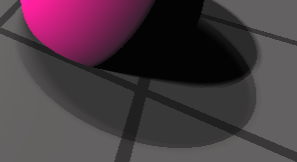
\includegraphics[width=0.7\textwidth]{Plantilla-TFG-master/img/shadowArtifactZoom.png}
    \caption{Detalle de las fugas de luz al calcular sombras}
    \label{fig:artifactZoom}
\end{figure}

La diferencia con nuestro método actual radica en que se permite que el rayo penetre un poco la superficie para detectar los puntos que casi no son alcanzados por un rayo de luz. Por tanto, ahora para cada punto se tiene en cuenta si casi ha sido alcanzado y si casi no ha sido alcanzado por un rayo de luz. Para permitir que el rayo entre en la geometría basta con modificar la condición de ruptura sobre $sdf$ a un número negativo, con la precaución de siempre sumar una cantidad positiva a $d$, pues de lo contrario el trazado del rayo retrocedería. Fijando este valor a $-1$ la variable $sombra$ tendrá un valor en el rango $[-1,1]$ al salir del bucle, pero aún queremos obtener un valor entre $[0,1]$ para representar la cantidad de luz que recibe el punto. Para remapear $sombra$ a este rango podemos usar la función \texttt{smoothstep(a,b,x)} de GLSL, que interpola $x$ suavemente entre $0$ y $1$ en relación con los límites $a$ y $b$. En particular la interpolación que se lleva a cabo es la de Hermite, haciendo que la transición entre distintos puntos de sombra no sea lineal y parezca más natural. Podemos ver el algoritmo final en la \autoref{fig:sombras3} y los resultados que consigue en la \autoref{fig:sombras4}.

\begin{figure}[ht!]
    \centering
    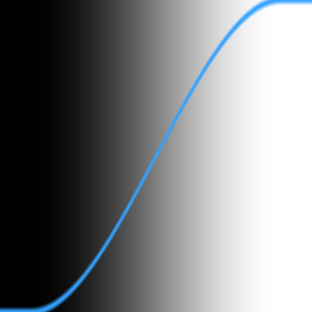
\includegraphics[width=0.3\textwidth]{Plantilla-TFG-master/img/smoothstep.png}
    \caption{Visualización de \texttt{smoothstep} \cite{smoothstep}}
    \label{fig:miss}
\end{figure}

\begin{figure}[ht!]
    \centering
   \begin{algorithm}[H]
        \caption{CalcularSombras}
            \KwData{punto $p_0$, dirección de luz $l_i$, tamaño de luz $k$}
            \KwResult{valor en el rango $[0,1]$ representando la cantidad de sombra recibida en $p_0$}
            $sombra \gets 1$
            
            $d \gets \delta$ \Comment{distancia actual}
            
            \For{i $\in$ MAX\_ITERACIONES} {
                $p \gets p_o + d \cdot v$
                
                $sombra \gets \Min(res, k\cdot \frac{sdf}{d})$
                
                $sdf \gets \phi(p)$

                $d \gets d + \vert sdf\vert$
                
                \If{$sombra < -1 $ \textbf{OR} $d > MAX\_DISTANCIA$}{
                   \textbf{break}
                } 
            }

            \Return{$smoothstep(-1,1,sombra)$}
    \end{algorithm}

    \caption{Cálculo de sombras suavizadas mejorado}
    \label{fig:sombras3}
\end{figure}

\begin{figure}[ht!]
    \centering
    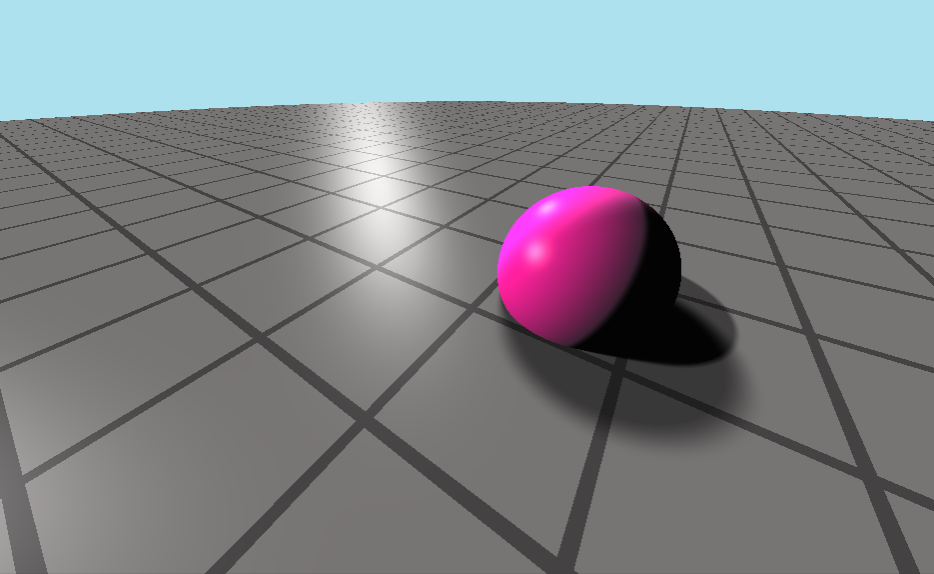
\includegraphics[width=\textwidth]{Plantilla-TFG-master/img/shadowSoft.png}
    \caption{Resultado final del cálculo de sombras}
    \label{fig:sombras4}
\end{figure}



\subsection{Oclusión ambiental}
Al añadir sombras los objetos están mucho más integrados en la escena, pero todavía podemos conseguir un mayo grado de cohesión. En el estado actual de la escena aún hay puntos que no es convincente que reciban luz pero se encuentran totalmente iluminados. Un ejemplo son los puntos de intersección entre la esfera y el suelo. Uno esperaría que poca luz fuera capaz de alcanzar un espacio tan cóncavo, pues la propia geometría de la esfera y el suelo ocluirían la luz. Este fenómeno recibe el nombre de \textbf{oclusión ambiental}, y de nuevo gracias a los SDF nos resultará muy fácil y computacionalmente barato simularlo.\newline

Cuando se trabaja con geometría de polígonos, una de las técnicas más comunes es la oclusión ambiental del espacio de pantalla, o SSAO por sus siglas en inglés. En su versión más básica esta solución usa la información del fotograma actual para consultar por cada píxel el \textif{buffer} de profundidad o \textit{deph buffer} de los píxeles cercanos. Con esta información realiza una aproximación de las características de la geometría en ese entorno y deduce la cantidad de luz que debería poder pasar. El principal problema de esta y otras técnicas basadas en el espacio de pantalla es que al no usar la información real de la geometría, los resultados obtenidos varían según la orientación de la cámara, posición relativa de los objetos en pantalla, etc. Otro método basado en espacio de pantalla que pone de manifiesto este problema es el de los reflejos de espacio de pantalla o SSR, que suele ser usado para simular reflejos como los del agua o espejos en videojuegos. Al usar el mismo principio que SSAO, solo podrá reflejar correctamente los píxeles que estén dibujados en pantalla. Esta limitación hace que cuando un objeto ocluye a otro este no se puede reflejar correctamente y se generen reflejos erróneos como se muestra en la \autoref{fig:ssrVS}, o que si un objeto no aparece en pantalla directamente no sea reflejado, como se representa en la \autoref{fig:ssrEsquema}.

\begin{figure}[!h]
     \begin{minipage}[c]{0.49\linewidth}
        \centering
        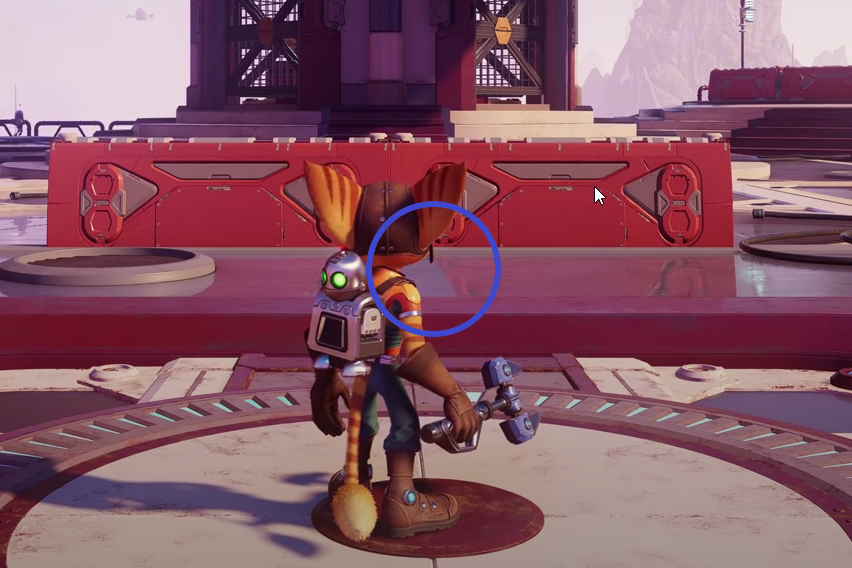
\includegraphics[width=0.98\textwidth]{Plantilla-TFG-master/img/ssr_on.png}
        \caption{SSR}
     \end{minipage}
     \begin{minipage}[c]{0.49\linewidth}
        \centering
        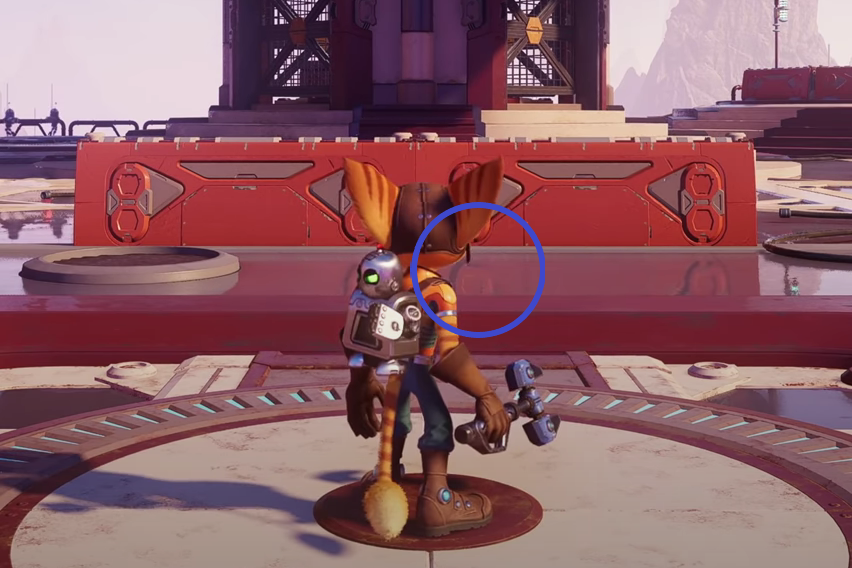
\includegraphics[width=0.98\textwidth]{Plantilla-TFG-master/img/ssr_off.png}
        \caption{\textit{Raytracing}}
     \end{minipage}
     \caption{Videojuego Ratchet \& Clank: Una dimensión aparte usando SSR y \textit{raytracing} \cite{ratchet}}
     \label{fig:ssrVS}
\end{figure}

\begin{figure}[!h]
     \begin{minipage}[c]{0.49\linewidth}
        \centering
        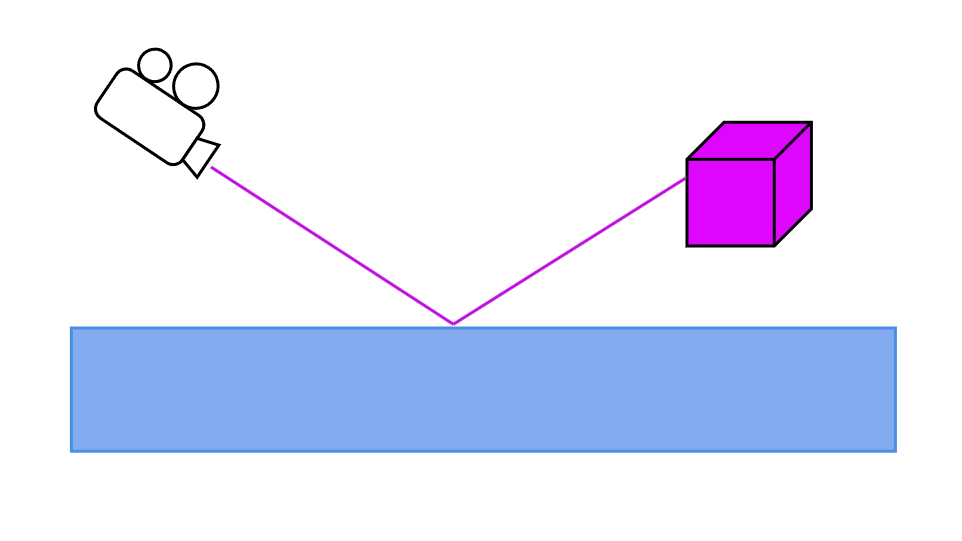
\includegraphics[width=0.9\textwidth]{Plantilla-TFG-master/img/ssr2.png}
        \caption{Reflejo detectado}
     \end{minipage}
     \begin{minipage}[c]{0.49\linewidth}
        \centering
        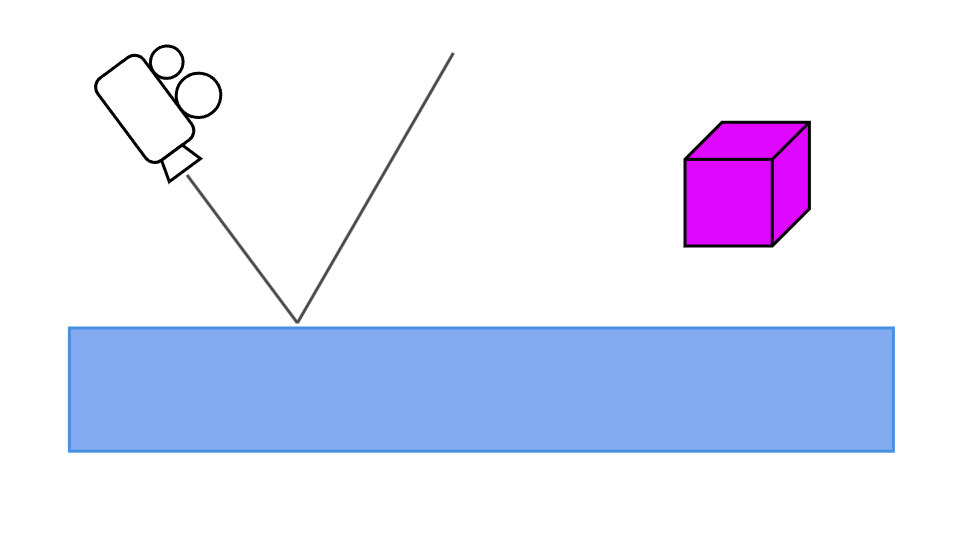
\includegraphics[width=0.9\textwidth]{Plantilla-TFG-master/img/ssr3.png}
        \caption{Reflejo no detectado}
     \end{minipage}
     \caption{Reflejos en agua con SSR}
     \label{fig:ssrEsquema}
\end{figure}

La solución a estos problemas cuando se trabaja con vértices es el uso de técnicas más avanzadas y computacionalmente costosas como el \textit{raytracing}. La buena noticia es que al estar usando SDFs nosotros podremos usar la información real de la geometría de nuestra escena. Obtendremos por tanto información más precisa, y además de forma muy barata, ya que requeriremos de muchas menos evaluaciones del SDF que el algoritmo de \textit{spheretracing}. La técnica que vamos a usar fue ideada por Alex Evans en 2006 \cite{ao}, y se conoce como \textbf{oclusión ambiental muestreada por la normal}.\newline

El método se basa en dado un punto $p\in S_{\phi}$ evaluar el SDF en varios puntos del vector normal $N_p$ a distancias $d_i$ de $p$ para obtener la información de la geometría cercana. Si en el entorno de $p$ hay geometría que le esté obstruyendo la llegada de luz, en alguna de estas evaluaciones se obtendrá un valor menor que $d_i$, mientras que de lo contrario uno esperaría que
\begin{equation*}
    \phi(p + d_i N_p) = d_i,
\end{equation*}
ya que eso significaría que el punto más cercano a $p$ de $S_{\phi}$ es el propio $p$. Así, si hacemos $M$ evaluaciones igualmente espaciadas a lo largo de $N_p$, consideraremos que el punto $p$ no está ocluido si
\begin{equation*}
    \sum_{i=1}^M \phi\Big(p + \frac{i}{M} N_p\Big) - \sum_{i=1}^M \frac{i}{M} = 0.
\end{equation*}
\begin{figure}[ht!]
    \centering
    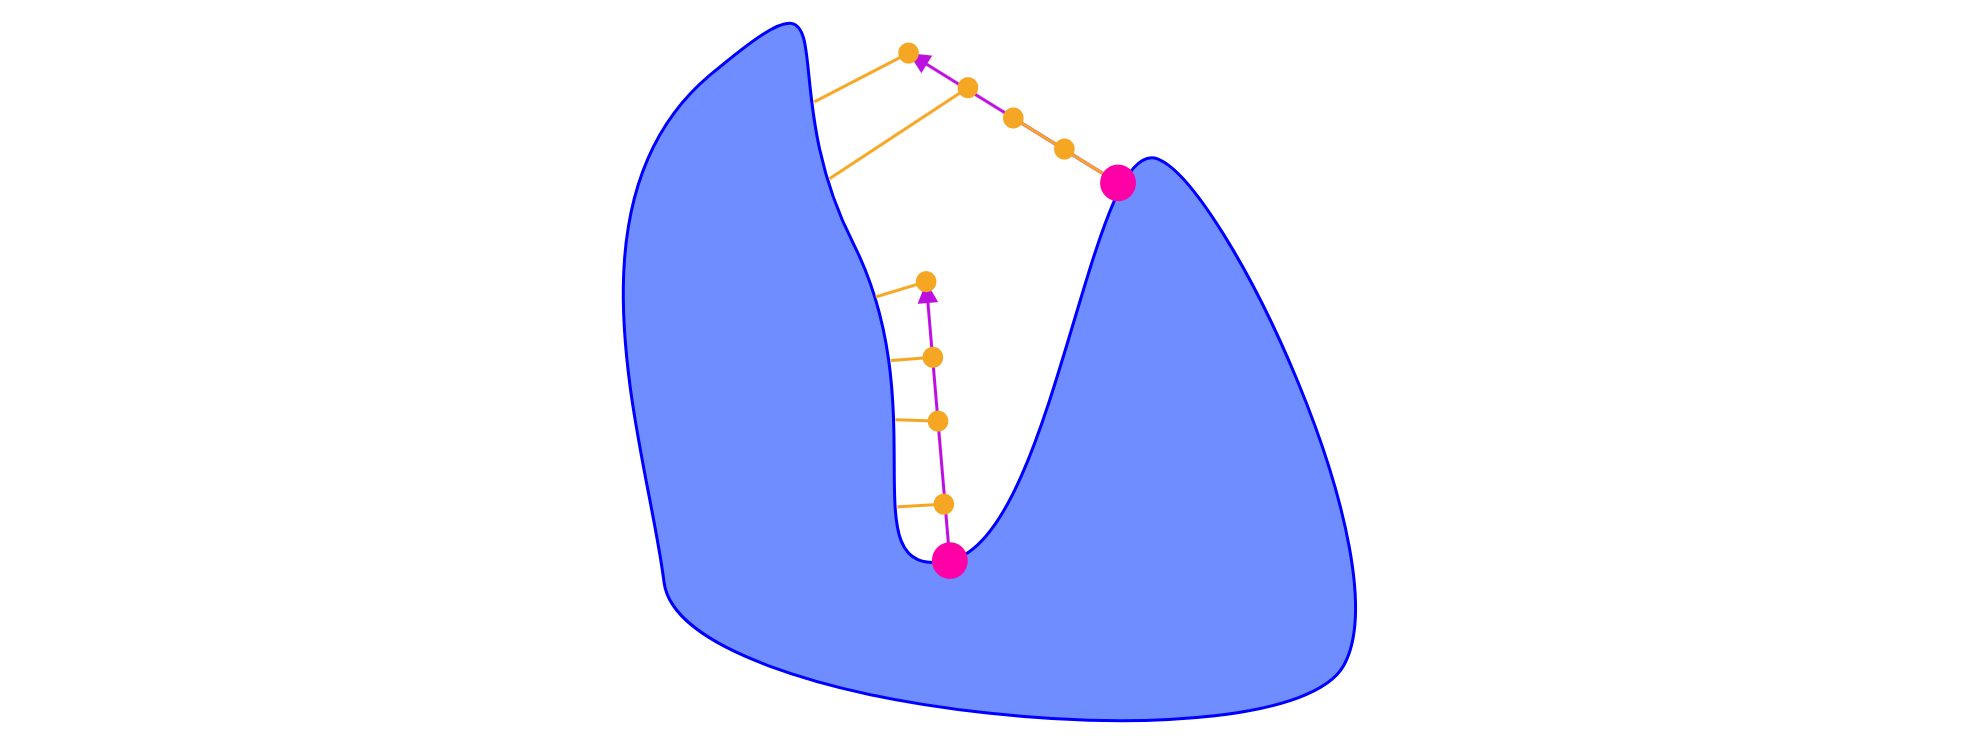
\includegraphics[width=\textwidth]{Plantilla-TFG-master/img/diagramaAO.png}
    \caption{Cálculo de oclusión ambiental muestreada por la normal}
    \label{fig:sombras4}
\end{figure}
Cuanto mayor sea este valor (no puede ser menor que $0$ por definición de SDF) menos luz será capaz de alcanzar $p$. Así, podemos representar la cantidad de luz ocluida como
\begin{equation*}
    \sum_{i=1}^M \frac{1}{2^i}\cdot \left(\frac{i}{M} - \phi\Big(p + \frac{i}{M} N_p\Big)\right)\in [0,1].
\end{equation*}
El hecho de que esté valor esté acotado en $[0,1]$ viene de que suponemos que $\Vert N_p\Vert = 1$, de forma que
\begin{equation*}
    \phi\left(p + \frac{i}{M} N_p\right) \le 1,
\end{equation*}
ya que siempre habrá algún punto a lo largo de $N_p$ que esté a una unidad o menos de distancia de $p$: él mismo. Por otro lado, hemos usado la exponencial para dar más peso sobre el resultado final a aquellos puntos más cercanos a $p$.\newline

Con esto ya podemos obtener la nueva versión del método \texttt{DibujarSuperficie} que tiene en cuenta la oclusión ambiental descrita en la \autoref{fig:dibujarAO}. En ella hemos introducido una pequeña optimización \cite{ao_opt} cambiando el índice del bucle para no tener que calcular una división en cada iteración. Otra posible optimización sería sustituir la potencia por un un flotante que fuéramos multiplicando por un factor menor que $1$ en cada iteración. Finalmente, podemos apreciar los resultados obtenidos en la \autoref{fig:resAO}, donde para valores tan pequeños de $M$ como $2$ o $4$ ya conseguimos resultados más que convincentes.

% donde hemos usado la exponencial para asegurar que $ao\in [0,1]$, que cuando no haya oclusión obtengamos $ao=1$ y que el resultado tenga un aspecto más natural. Además $k$ controlará la intensidad del efecto. Sin embargo preferiremos ganar algo de eficiencia simulando el comportamiento de la exponencial con una constante que iremos multiplicando por sí misma en cada iteración. Así, la nueva versión del método \texttt{DibujarSuperficie} será el descrito en la \autoref{fig:dibujarAO}.

\begin{figure}
    \centering
        
    \begin{algorithm}[H]
        \caption{DibujarSupercicie}
            \KwData{punto $p$, dirección del rayo $v$, distancia $\phi(p)$}
            $L \gets L_A + L_E$ \Comment{Radiancia final}
            \For{$i \in \{1,\dots, n\}$} {
    
                
                \Comment{ ··· }
                $N_p \gets CalcularNormal(p)$
                
                $sombras \gets CalcularSombras(p, l_i)$
                
                $ao \gets CalcularAO(p, N_p)$
    
                $L \gets L + S_i\cdot (f_{ra} + f_{rd} + f_{re})\cdot sombras \cdot ao$
            }
    
            \Return{$L$}
    \end{algorithm}
    
    \begin{algorithm}[H]
        \caption{CalcularAO}
            \KwData{punto $p$, vector normal $N_p$}
            \KwResult{$ao \in [0,1]$}
            $ao \gets 1$
                    
            $increment \gets \nicefrac{1}{M}$
            
            $i\gets increment$
        
            \While{$i<1$}{
                $sdf \gets \phi(p + iN_p)$
                
                $ao \gets ao - 2^{-iM}\cdot (i-sdf)$
    
                $i\gets i+increment$
            }
                
            \Return{$ao$}
    \end{algorithm}
    
    \caption{Cálculo de oclusión ambiental}
    \label{fig:dibujarAO}
\end{figure}


\begin{figure}[!h]
     \begin{minipage}[c]{0.49\linewidth}
        \centering
        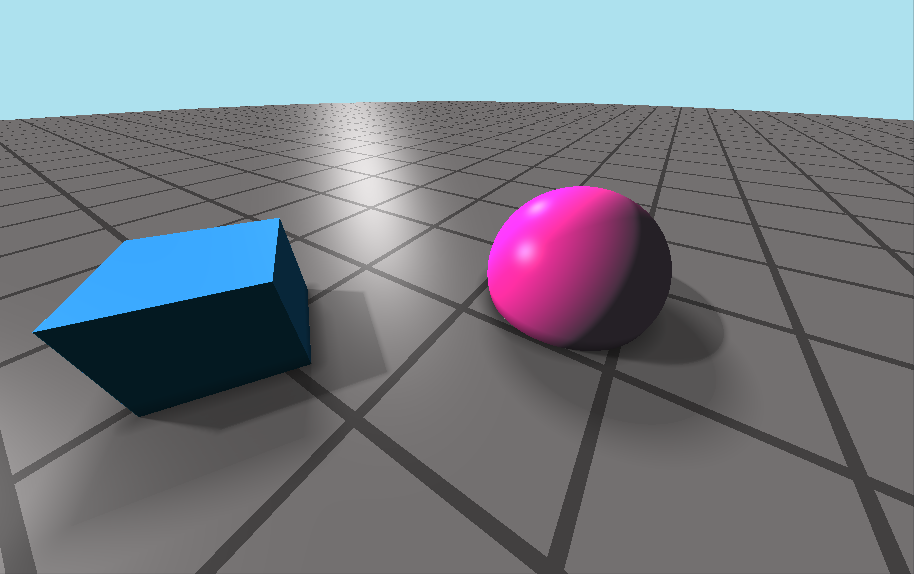
\includegraphics[width=0.98\textwidth]{Plantilla-TFG-master/img/ao2.png}
        \caption{$M=2$}
     \end{minipage}
     \begin{minipage}[c]{0.49\linewidth}
        \centering
        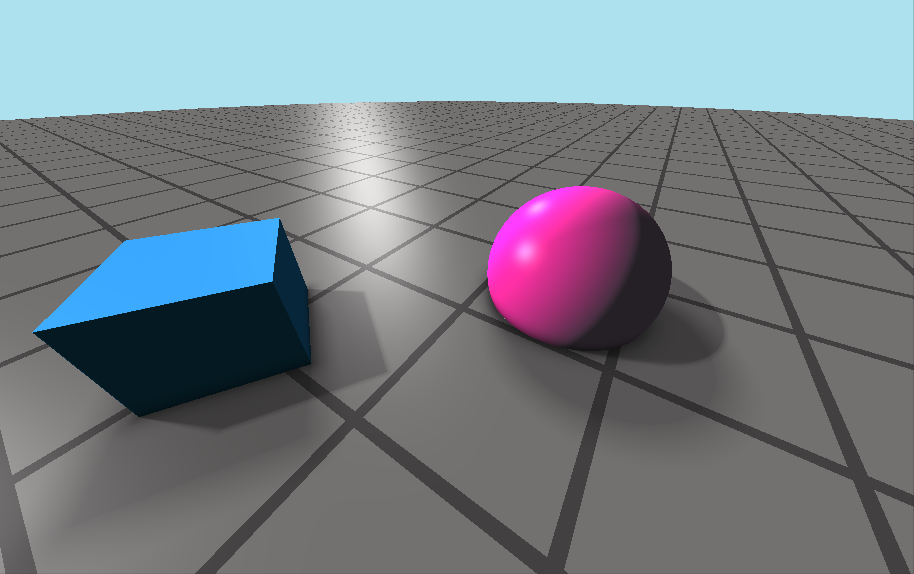
\includegraphics[width=0.98\textwidth]{Plantilla-TFG-master/img/ao4.png}
        \caption{$M=4$}
     \end{minipage}
     \caption{Resultado del cálculo de oclusión ambiental}
     \label{fig:resAO}
\end{figure}

\section{\textit{Antialiasing}}\label{sec:aa}
Vamos a introducir una última mejora en la forma en la que generamos la imagen. Un defecto típico en computación gráfica es el conocido como \textbf{\textit{aliasing}}. Este se caracteriza por la presencia de dientes de sierra en lineas curvas o diagonales, y en nuestro caso se puede apreciar muy fácilmente en los bordes del cubo y en la cuadrícula del suelo en la distancia (\autoref{subfig:noAA}). En el mercado actual existen multitud de alternativas como solución a este problema. Algunos ejemplos son FXAA, basado en espacio de pantalla, o SSAA y MSAA, que usan la técnica del \textbf{supermuestreo} o \textbf{\textit{supersampling}} junto con filtros de suavizado. Nosotros implementaremos una versión de SSAA (\textit{Supersampling Anti-Aliasing}), pero antes debemos entender por qué aparece el problema del \textit{aliasing} en primer lugar. \newline

Toda pantalla tiene resolución finita, y por tanto la definición con la que puede mostrar la información es limitada. Al realizar la proyección sobre la pantalla puede ocurrir que una primitiva no ocupe un píxel completo, y como cada píxel solo puede mostrar un único color hay que elegir algún criterio para determinar qué hacer en esos casos. El más común es considerar que el píxel pertenece a la primitiva si su proyección cubre el centro del píxel. En nuestro caso esto se traducía en trazar el rayo a través del centro del píxel en el algoritmo de \textit{spheretracing}. Al hacer esta aproximación es cuando aparecen los dientes de sierra, pues a no ser que se trate de una línea totalmente vertical u horizontal, es como si intentásemos construir una rampa con escalones.\newline

Lo cierto es que no podemos hacer desaparecer este problema, pues es algo intrínseco de la naturaleza discreta de las pantallas y los sistemas de muestreo. En nuestro caso esto último se traduce en que no podemos trazar infinitos rayos. No obstante, lo que sí podemos hacer es tratar de disimularlo. En lugar de tomar una decisión binaria de si un píxel debe ser de un color u otro podemos intentar tener en cuenta la aportación de otras primitivas que estén cercanas dentro del píxel aunque no ocupen su centro. Una primera idea podría ser que una vez asignado un color a un píxel se hiciera la media con sus píxeles vecinos para así generar una transición suave entre ellos. Sin embargo este acercamiento presenta dos grandes inconvenientes:
\begin{itemize}
    \item Estaríamos perdiendo parte de la información original, y por ende, haciendo la imagen más borrosa.
    \item El responsable de asignar el color de cada píxel es una instancia del \textit{fragment shader}, y como ya comentamos, los \textit{shaders} son programas independientes y no tienen información sobre el resto de instancias. Por tanto este método sería de postprocesado, es decir, sería ejecutado una vez hubiera sido generada la imagen.
    
\end{itemize}

De esto podemos sacar la conclusión de que la solución debe ser local a cada píxel, y de ser posible que no conlleve la pérdida de información. La opción de hacer una media entre varias muestras de píxeles sigue pareciendo razonable, lo que nos lleva a la idea detrás de SSAA: tomar más muestras dentro de cada píxel. Para ello, tendremos que trazar rayos por más puntos dentro del píxel, esto es, dibujar la imagen con mayor resolución, de donde viene el nombre de supermuestreo. El patrón en el que tomamos las nuevas muestras es de nuestra elección. En la \autoref{fig:patrones} se muestran algunos patrones comunes, de los cuales optaremos por el uniforme por su sencillez y porque proporciona resultados bastante buenos en general. El número de evaluaciones también está a nuestra elección, pero no hay que olvidar el factor del rendimiento, ya que usando este patrón el número de rayos crece exponencialmente por cada nuevo nivel adicional de precisión.
\newline

\begin{figure}[htbp]
    \centering
    \begin{subfigure}[b]{0.25\textwidth}
        \centering
        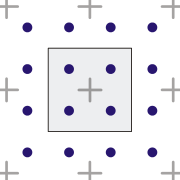
\includegraphics[width=\textwidth]{Plantilla-TFG-master/img/aa1.png}
        \caption{Uniforme}
    \end{subfigure}
    \hfill
    \begin{subfigure}[b]{0.25\textwidth}
        \centering
        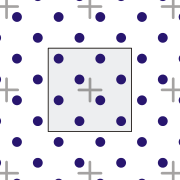
\includegraphics[width=\textwidth]{Plantilla-TFG-master/img/aa2.png}
        \caption{Rejilla girada}
    \end{subfigure}
    \hfill
    \begin{subfigure}[b]{0.25\textwidth}
        \centering
        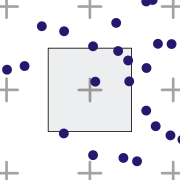
\includegraphics[width=\textwidth]{Plantilla-TFG-master/img/aa3.png}
        \caption{Aleatorio}
    \end{subfigure}
    
    \medskip
    
    \begin{subfigure}[b]{0.25\textwidth}
        \centering
        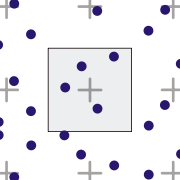
\includegraphics[width=\textwidth]{Plantilla-TFG-master/img/aa4.png}
        \caption{\textit{Quasi-Monte Carlo}}
    \end{subfigure}
    \hfill
    \begin{subfigure}[b]{0.25\textwidth}
        \centering
        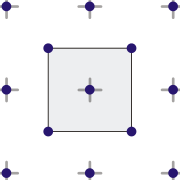
\includegraphics[width=\textwidth]{Plantilla-TFG-master/img/aa5.png}
        \caption{HRAA}
    \end{subfigure}
    \hfill
    \begin{subfigure}[b]{0.25\textwidth}
        \centering
        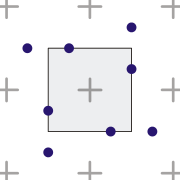
\includegraphics[width=\textwidth]{Plantilla-TFG-master/img/aa6.png}
        \caption{\textit{Flipquad}}
    \end{subfigure}
    \caption{Patrones de supermuestreo \cite{supersamp}}
    \label{fig:patrones}
\end{figure}

Modificar por dónde pasan los rayos dentro de cada píxel equivale a cambiar cómo calculamos los \texttt{uv}. Llamaremos a partir de ahora $AA$ al factor de escalado de la imagen, de forma que por cada píxel haremos pasar $4^{AA-1}$ rayos. Para hallar los nuevos puntos de muestra bastará con subdividir el píxel en $AA^2$ cuadrantes y quedarnos con el centro de cada uno. Si recordamos que $v_{frag}$ devuelve las coordenadas del centro del píxel, que el ancho y alto del píxel es una unidad, y que tenemos que hacer $AA$ subdivisiones en cada eje, es evidente que podemos obtener los nuevos puntos de muestra desplazando el origen usual del píxel la cantidad
\begin{equation*}
    offset_{m,n} = (m+\nicefrac{1}{2},n+\nicefrac{1}{2}))\cdot subdivision - \left( \frac{lado}{2}, \frac{lado}{2}\right) = \frac{ (m+\nicefrac{1}{2},n+\nicefrac{1}{2}))}{AA} - \left( \frac{1}{2}, \frac{1}{2}\right),
\end{equation*}
donde $m,n\in \{0,\dots, AA-1\}$.\newline
\begin{figure}[!h]
    \centering
    \begin{subfigure}[b]{0.4\textwidth}
        \centering
        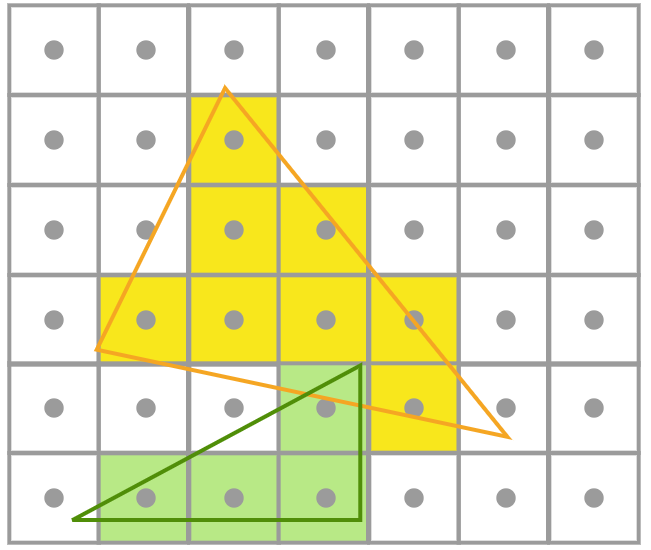
\includegraphics[width=\textwidth]{Plantilla-TFG-master/img/grid1.png}
        \caption{$AA = 1$}
    \end{subfigure}
    \hspace{15pt}
    \begin{subfigure}[b]{0.4\textwidth}
        \centering
        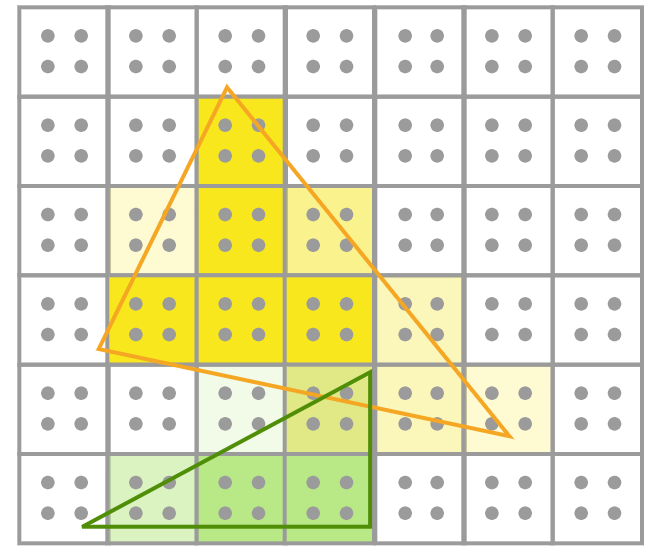
\includegraphics[width=\textwidth]{Plantilla-TFG-master/img/grid2.png}
        \caption{$AA = 2$}
    \end{subfigure}
    \hfill
     \caption{\textit{Antialiasing} para diferentes valores de $AA$}
\end{figure}

Para trasladar esto a nuestro \textit{fragment shader} tan solo habrá que realizar un doble bucle e ir sumando el color obtenido por \textit{spheretracing} en una variable que luego ponderaremos por el número total de muestras, $AA^2$. La nueva versión del \textit{fragment shader} se describe en la \autoref{fig:divPixel}.

\begin{figure}[ht!]
    \centering
    \begin{minipage}{0.69\textwidth}
      \begin{algorithm}[H]
            \caption{Fragment Shader}
            \KwData{coordenadas de dispositivo $v_{frag}$ del píxel actual}
            \KwResult{color del píxel actual como terna RGBA $v_{col}$}
            $c_0 \gets $ posición de cámara en función de la entrada del ratón

            $l\gets $ punto de atención elegido por el usuario
            
            $color\gets (0,0,0)$
            
            \For{$m \in \{0,\dots, AA-1\}$}{
            \For{$n \in \{0,\dots, AA-1\}$}{
                $offset \gets \frac{(m,n)}{AA} - (0.25, 0.25)$\\[8pt]
                
                $uv \gets 2\cdot \frac{(v_{frag}+offset)- 0.5\cdot u\_resolution.xy}{u\_resolution.y}$\\[8pt]

                $r_d \gets (f_1\ \vert \ f_2\ \vert \ f_3)\cdot normalizar((uv_x, uv_y,-1))$\\[5pt]

                $color \gets color + spheretracing(c_0, r_d)$
                }
            }

            $color \gets color / AA^2$
            
            $v_{col} \gets (color_x, color_y, color_z, 1)$
        \end{algorithm}
    \end{minipage}%
    \hfill
    \begin{minipage}{0.31\textwidth}
        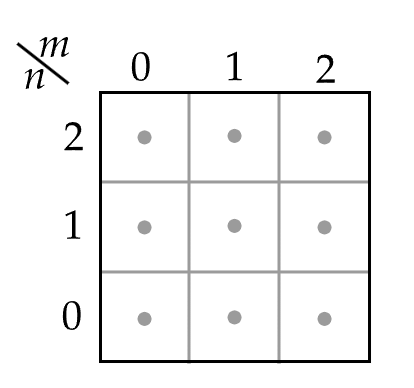
\includegraphics[width=\textwidth]{buclePixels.png}
    \end{minipage}
    \caption{Cuerpo del método \texttt{main} del \textit{fragment shader}}
    \label{fig:divPixel}
\end{figure}

Es evidente que $AA=1$ equivale a no aplicar \textit{antialiasing}, pero tendrá el efecto de desplazar la imagen medio píxel hacia abajo y a la izquierda, pues el único de cada píxel pasará por su esquina inferior. Por tanto, aunque no sea totalmente necesario, se puede añadir una comprobación para calcular los $uv$ como hacíamos originalmente en este caso. En la \autoref{fig:resAA} podemos ver que la pérdida de rendimiento no es en vano y obtenemos una imagen mucho más suave que la original. Sin embargo, no conviene tomar un valor de $AA$ mayor que $3$, pues generará mucha sobrecarga y la mejora no es muy apreciable. Finalmente y para concluir la sección, en el \autoref{ap:comparacionEscenas} podemos ver la construcción que hemos hecho de la escena paso a paso, viendo el efecto que ha tenido en el aspecto final cada técnica que hemos ido añadiendo.

\begin{figure}[htbp]
    \centering
    \begin{subfigure}[b]{0.3\textwidth}
        \centering
        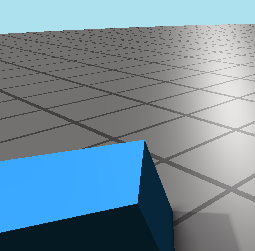
\includegraphics[width=\textwidth]{Plantilla-TFG-master/img/aa1_zoom.png}
        \caption{Detalle con $AA = 1$}
        \label{subfig:noAA}
    \end{subfigure}
    \hfill
    \begin{subfigure}[b]{0.3\textwidth}
        \centering
        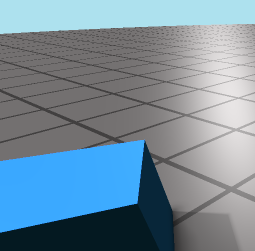
\includegraphics[width=\textwidth]{Plantilla-TFG-master/img/aa2_zoom.png}
        \caption{Detalle con $AA = 2$}
    \end{subfigure}
    \hfill
    \begin{subfigure}[b]{0.3\textwidth}
        \centering
        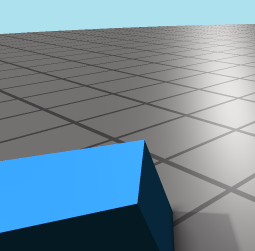
\includegraphics[width=\textwidth]{Plantilla-TFG-master/img/aa3_zoom.png}
        \caption{Detalle con $AA = 3$}
    \end{subfigure}

    \medskip
    
    \begin{subfigure}[b]{\textwidth}
        \centering
        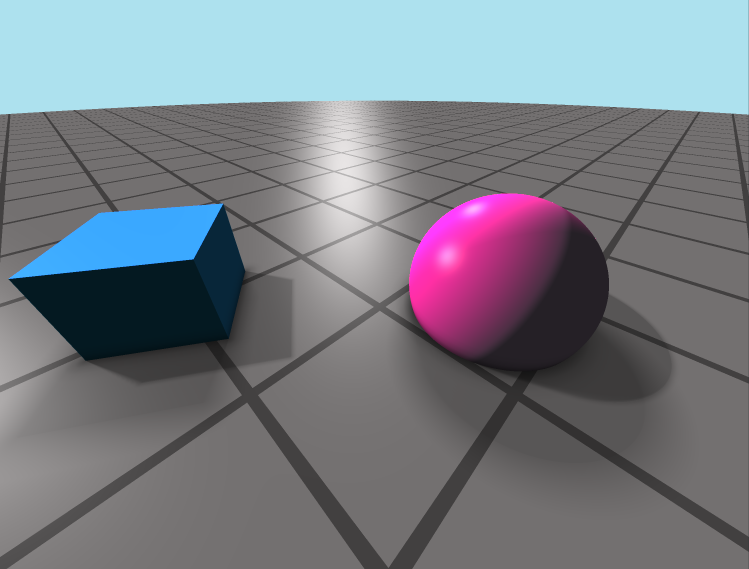
\includegraphics[width=\textwidth]{Plantilla-TFG-master/img/escena9_AA3.png}
        \caption{Escena completa con $AA=3$}
    \end{subfigure}
    
    \caption{Resultados de añadir \textit{antialiasing}}
    \label{fig:resAA}
\end{figure}





